%%%%%%%%%%%%%%%%%%%%%%%%%%%%%%%%%%%%%%%%%%%%%%%%%%%%%%%%%%%%%%%%%%%%%%%%%%%%%%%%%%
\begin{frame}[fragile]\frametitle{}
\begin{center}
{\Large Introduction}
\end{center}
\end{frame}


%%%%%%%%%%%%%%%%%%%%%%%%%%%%%%%%%%%%%%%%%%%%%%%%%%%%%%%%%%%%%%%%%%%%%%%%%%%%%%%%%%
\begin{frame}[fragile]\frametitle{Welcome}
  % \begin{center}
    % 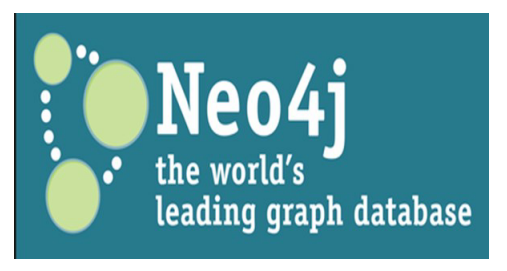
\includegraphics[width=0.4\textwidth]{neo4j32}
  % \end{center}
  \vspace{0.5em}
  \begin{itemize}
    \item Graphs are a powerful tool for modeling and analyzing complex relationships.
    \item In this presentation, we will explore the ubiquitous nature of graphs and how Neo4j's graph database can unlock their potential.
    \item Let's dive into the world of graphs!
  \end{itemize}
\end{frame}


%%%%%%%%%%%%%%%%%%%%%%%%%%%%%%%%%%%%%%%%%%%%%%%%%%%%%%%%%%%%%%%%%%%%%%%%%%%%%%%%%%
\begin{frame}[fragile]\frametitle{Graphs? Which one?}

  \begin{center}
    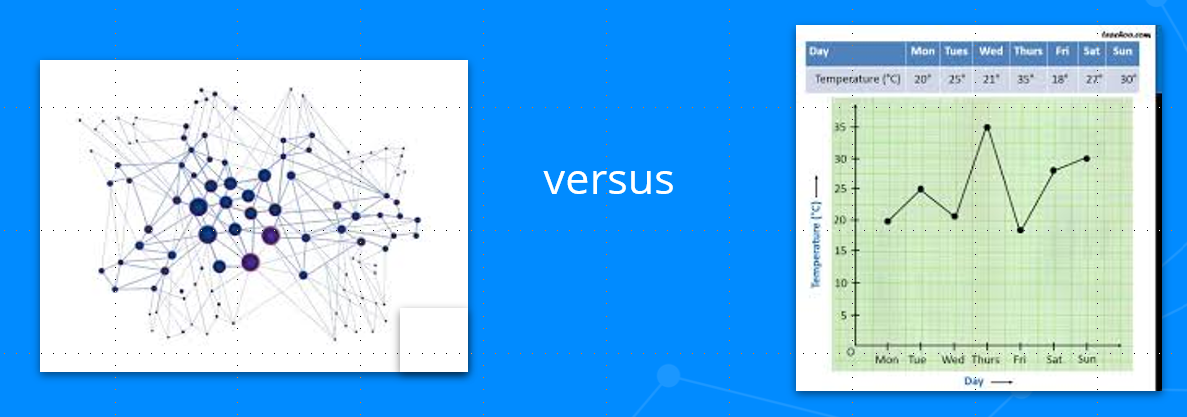
\includegraphics[width=\linewidth]{neo4j105}
  \end{center}

\end{frame}


%%%%%%%%%%%%%%%%%%%%%%%%%%%%%%%%%%%%%%%%%%%%%%%%%%%%%%%%%%%%%%%%%%%%%%%%%%%%%%%%%%
\begin{frame}[fragile]\frametitle{A graph is}
{\emph \ldots a set of discrete objects, each of which has some set of relationships with the other objects}

Euler: Can we take a walk to all 4 islands, without crossing any of the bridge twice?

Abstraction (Does size of islands matter?):

\begin{center}
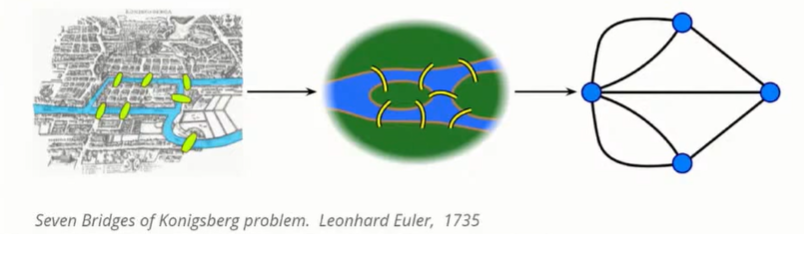
\includegraphics[width=\linewidth,keepaspectratio]{neo4j4}
\end{center}	  

Solution: No way!! What's the rule? [Ans: Homework!!]

{\tiny (Ref: Introduction to Neo4j - a hands-on crash course - neo4j)}
\end{frame}




%%%%%%%%%%%%%%%%%%%%%%%%%%%%%%%%%%%%%%%%%%%%%%%%%%%%%%%%%%%
\begin{frame}[fragile]\frametitle{ Graph-structured Data Are Ubiquitous }

\begin{center}
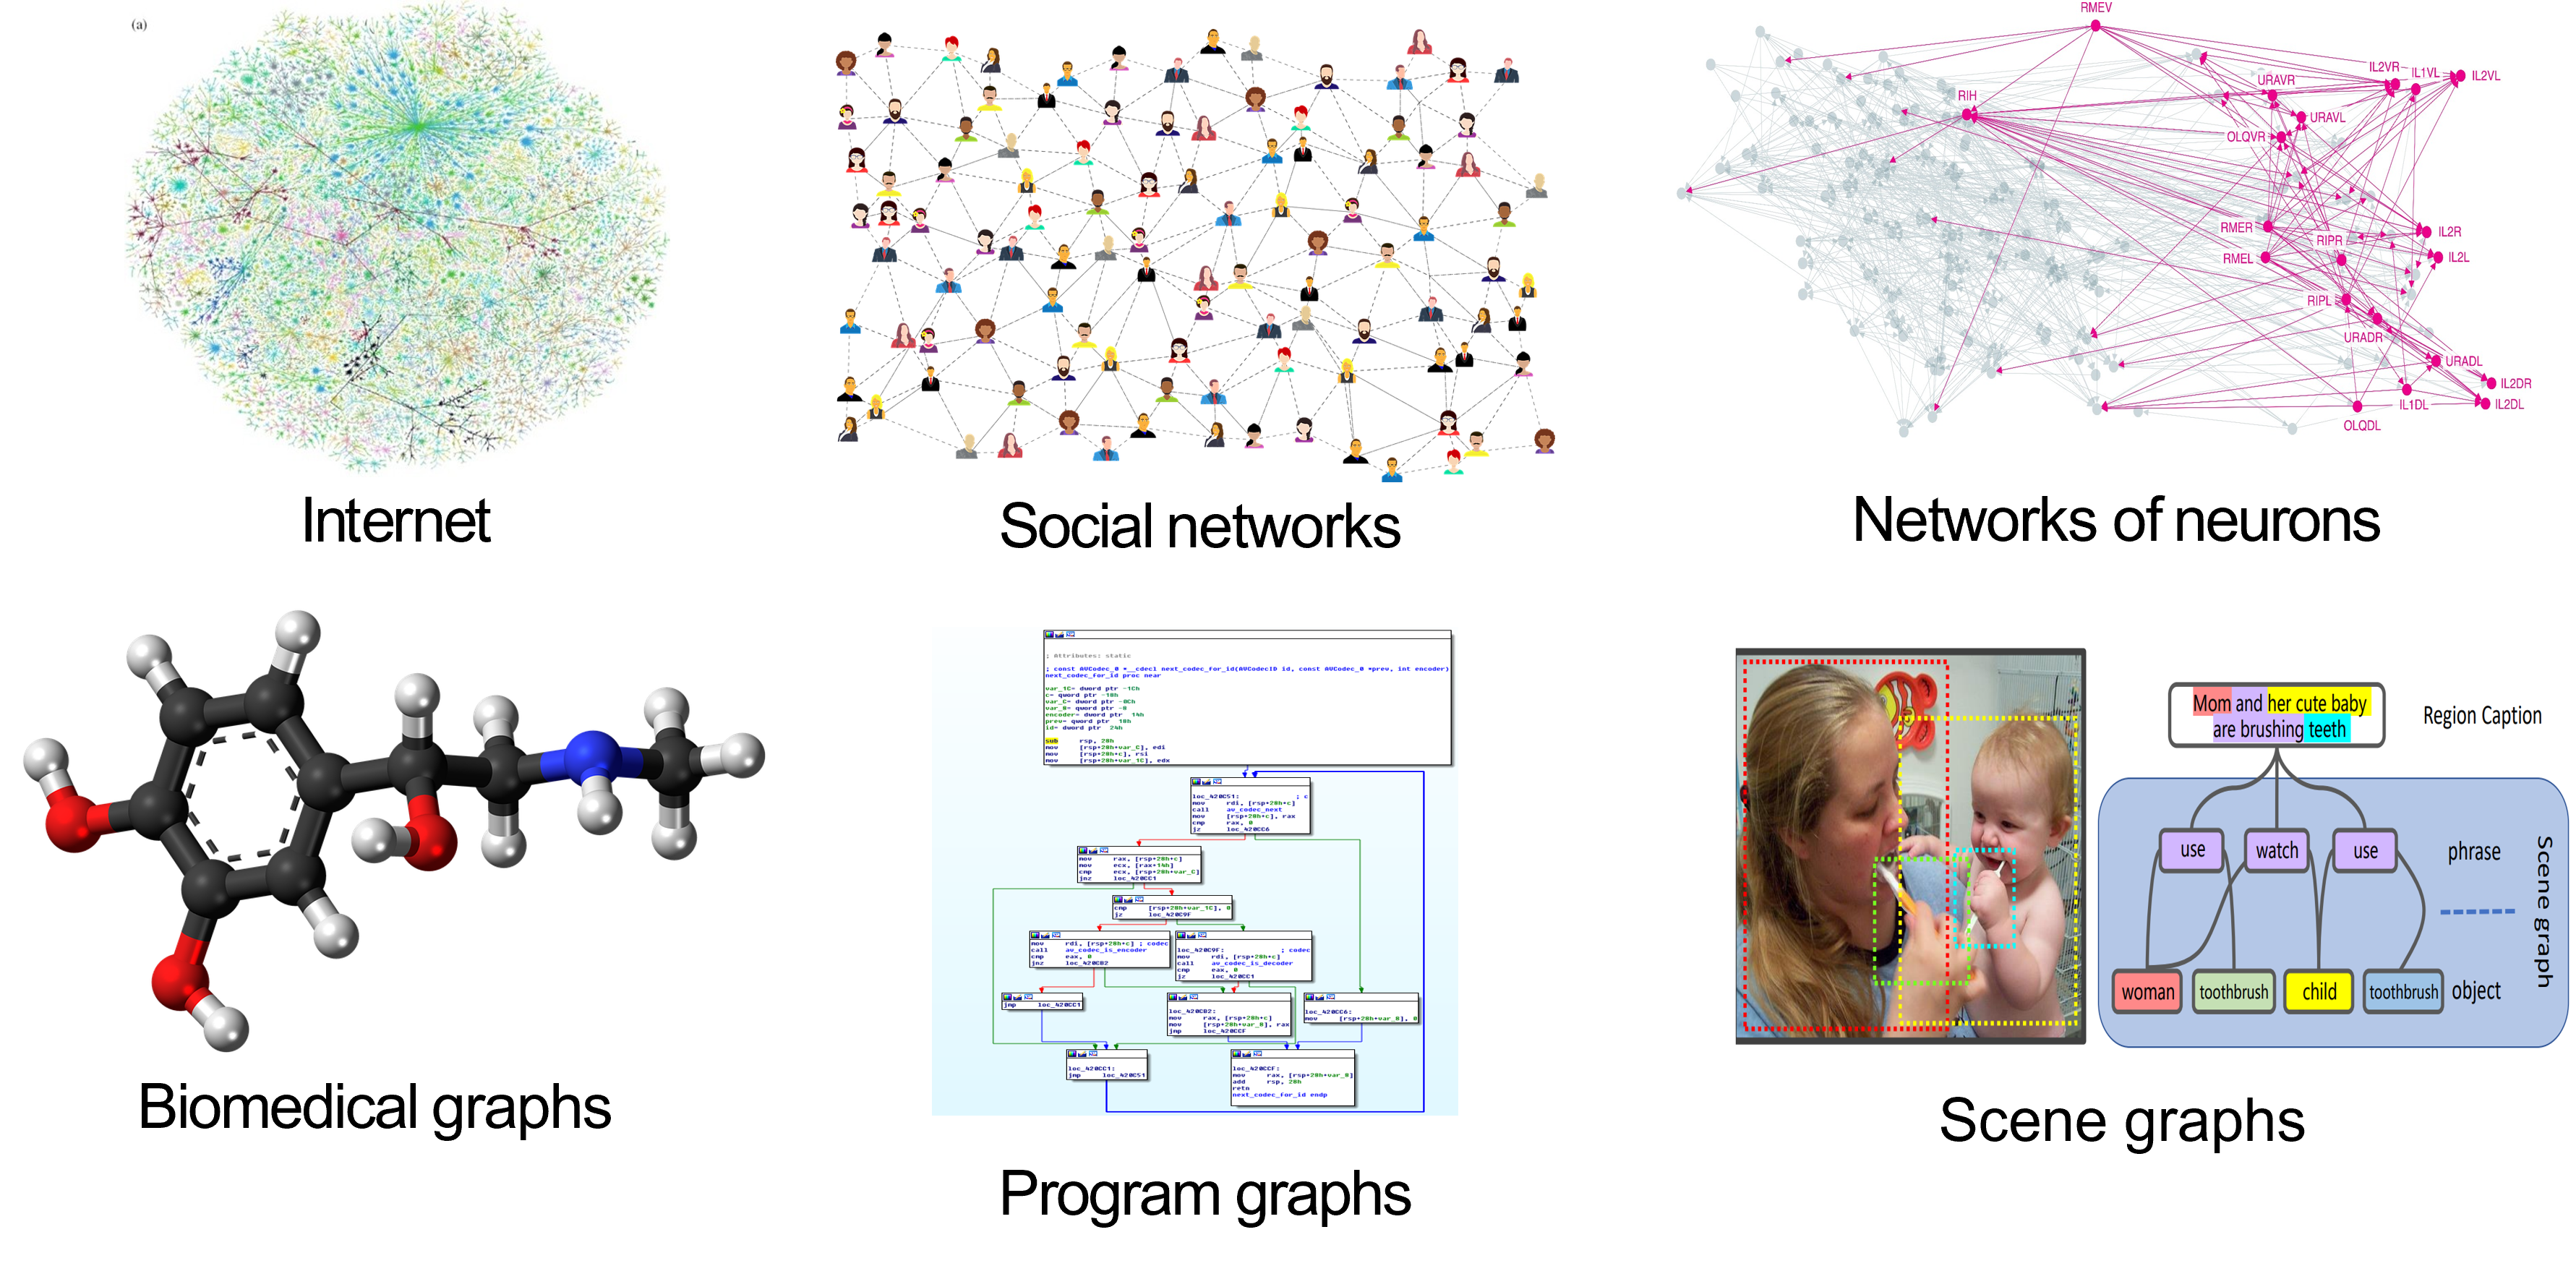
\includegraphics[width=\linewidth,keepaspectratio]{gnn1}
\end{center}	  

\end{frame}

%%%%%%%%%%%%%%%%%%%%%%%%%%%%%%%%%%%%%%%%%%%%%%%%%%%%%%%%%%%
\begin{frame}[fragile]\frametitle{}

\begin{center}
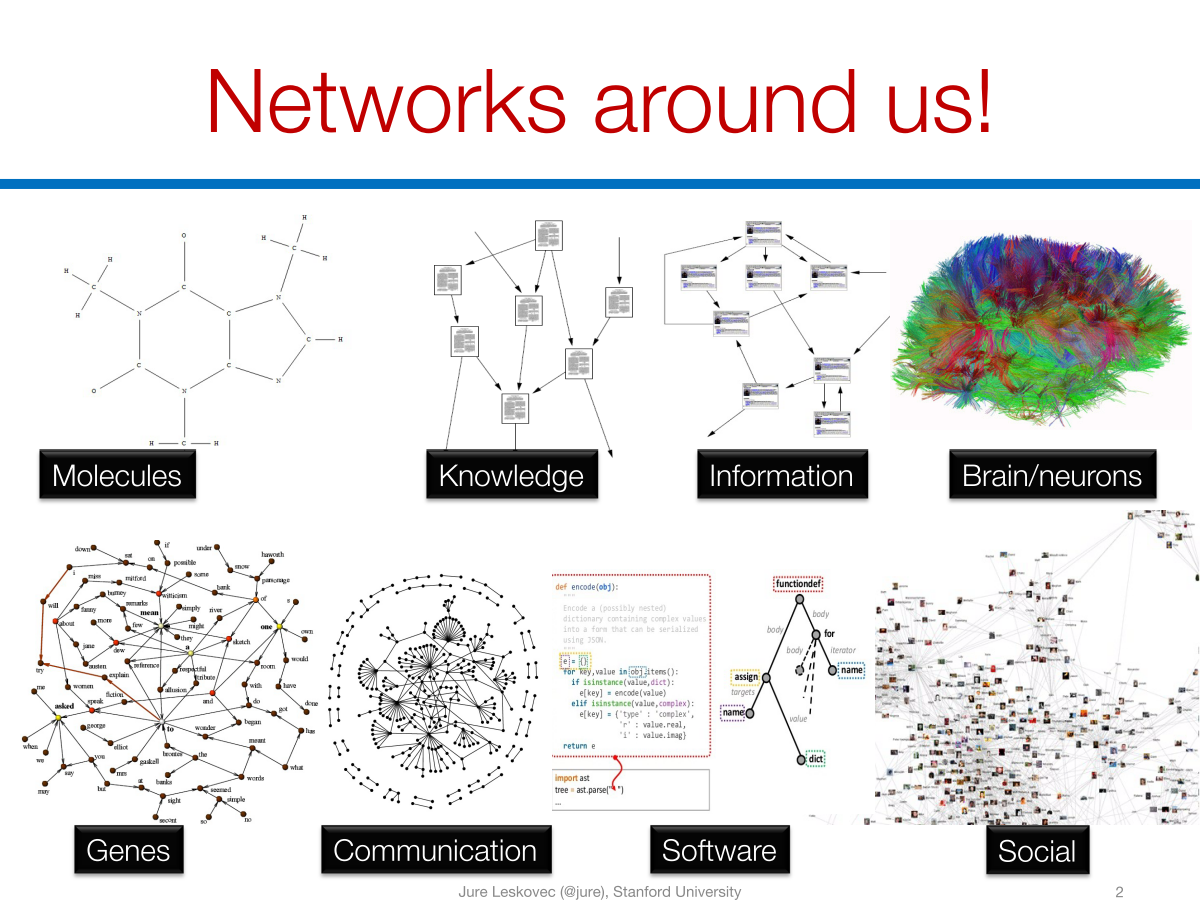
\includegraphics[width=\linewidth,keepaspectratio]{gnn2}
\end{center}	  

\end{frame}

%%%%%%%%%%%%%%%%%%%%%%%%%%%%%%%%%%%%%%%%%%%%%%%%%%%%%%%%%%%
\begin{frame}[fragile]\frametitle{}

\begin{center}
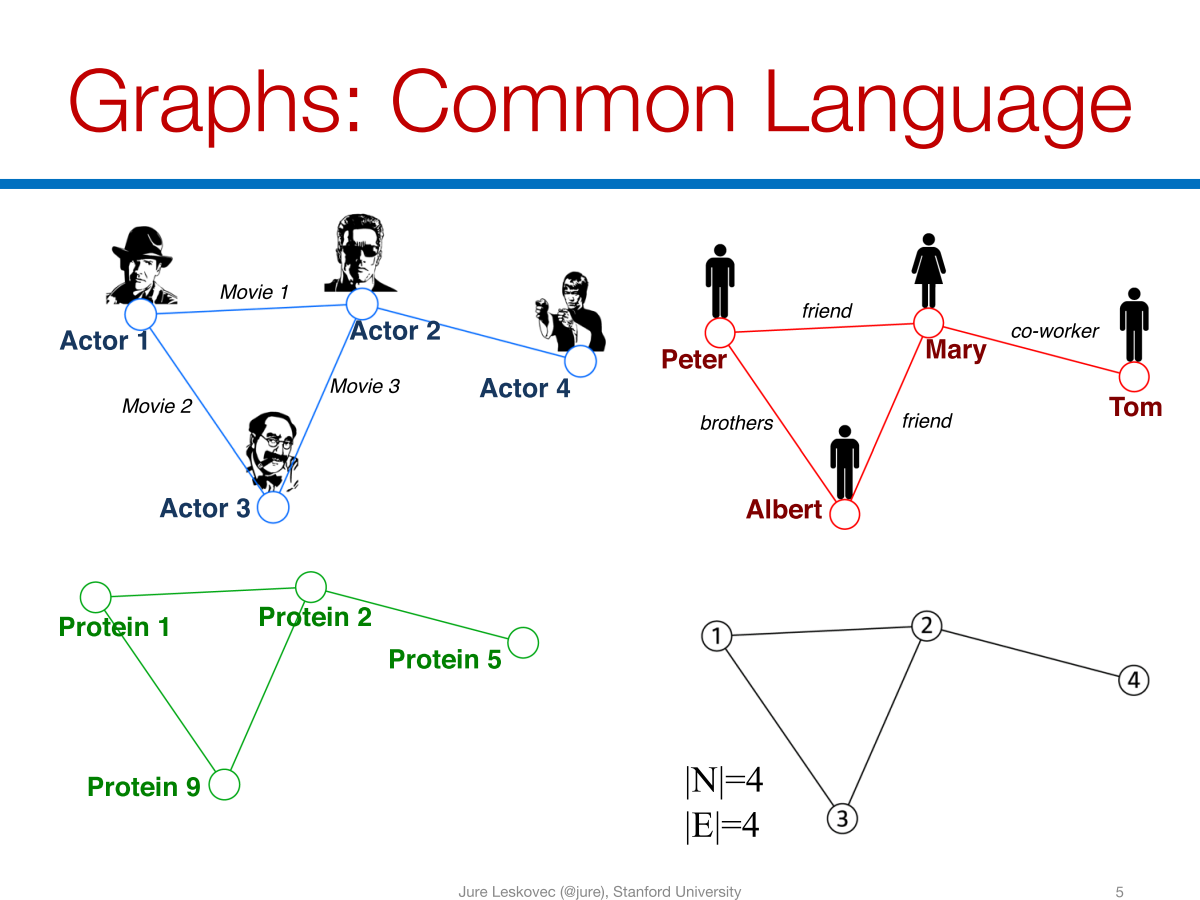
\includegraphics[width=\linewidth,keepaspectratio]{gnn3}
\end{center}	  

\end{frame}

%%%%%%%%%%%%%%%%%%%%%%%%%%%%%%%%%%%%%%%%%%%%%%%%%%%%%%%%%%%
\begin{frame}[fragile]\frametitle{Graphs are everywhere !}

\begin{center}
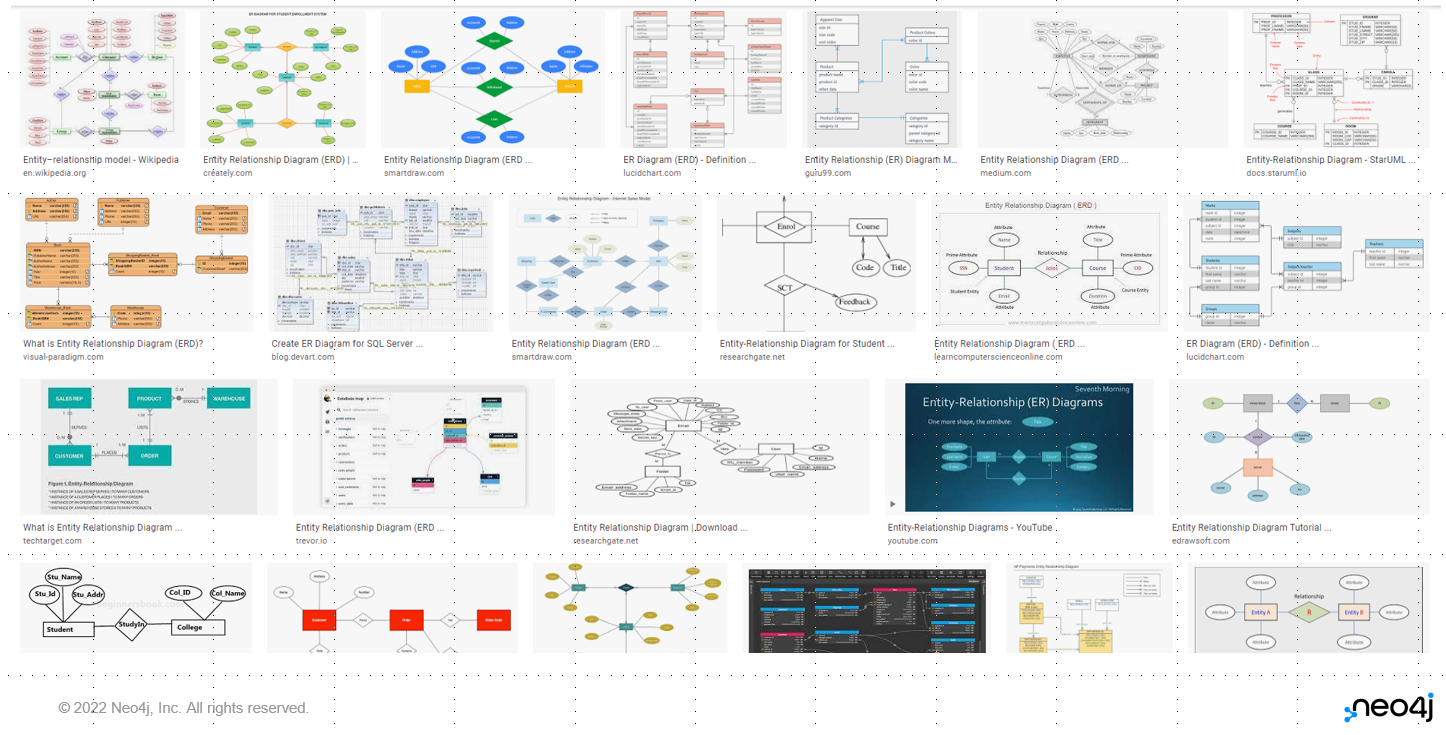
\includegraphics[width=\linewidth,keepaspectratio]{neo4j106}
\end{center}	  

\end{frame}

%%%%%%%%%%%%%%%%%%%%%%%%%%%%%%%%%%%%%%%%%%%%%%%%%%%%%%%%%%%%%%%%%%%%%%%%%%%%%%%%%%
\begin{frame}\frametitle{ Why do graphs matter? }

Across an organization, every department can benefit from graphs to answer questions 
like who or what is important, what should I do next, and what’s unusual about this?

\begin{center}
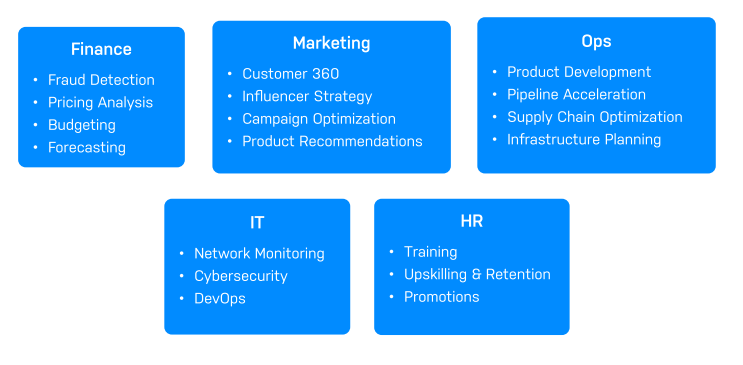
\includegraphics[width=\linewidth,keepaspectratio]{neo4j103}
\end{center}	  


{\tiny (Ref: 5 Graph Data Science Basics Everyone Should Know - neo4j)}
\end{frame}

%%%%%%%%%%%%%%%%%%%%%%%%%%%%%%%%%%%%%%%%%%%%%%%%%%%%%%%%%%%
\begin{frame}[fragile]\frametitle{Graphs: A Universal Language }

\begin{center}
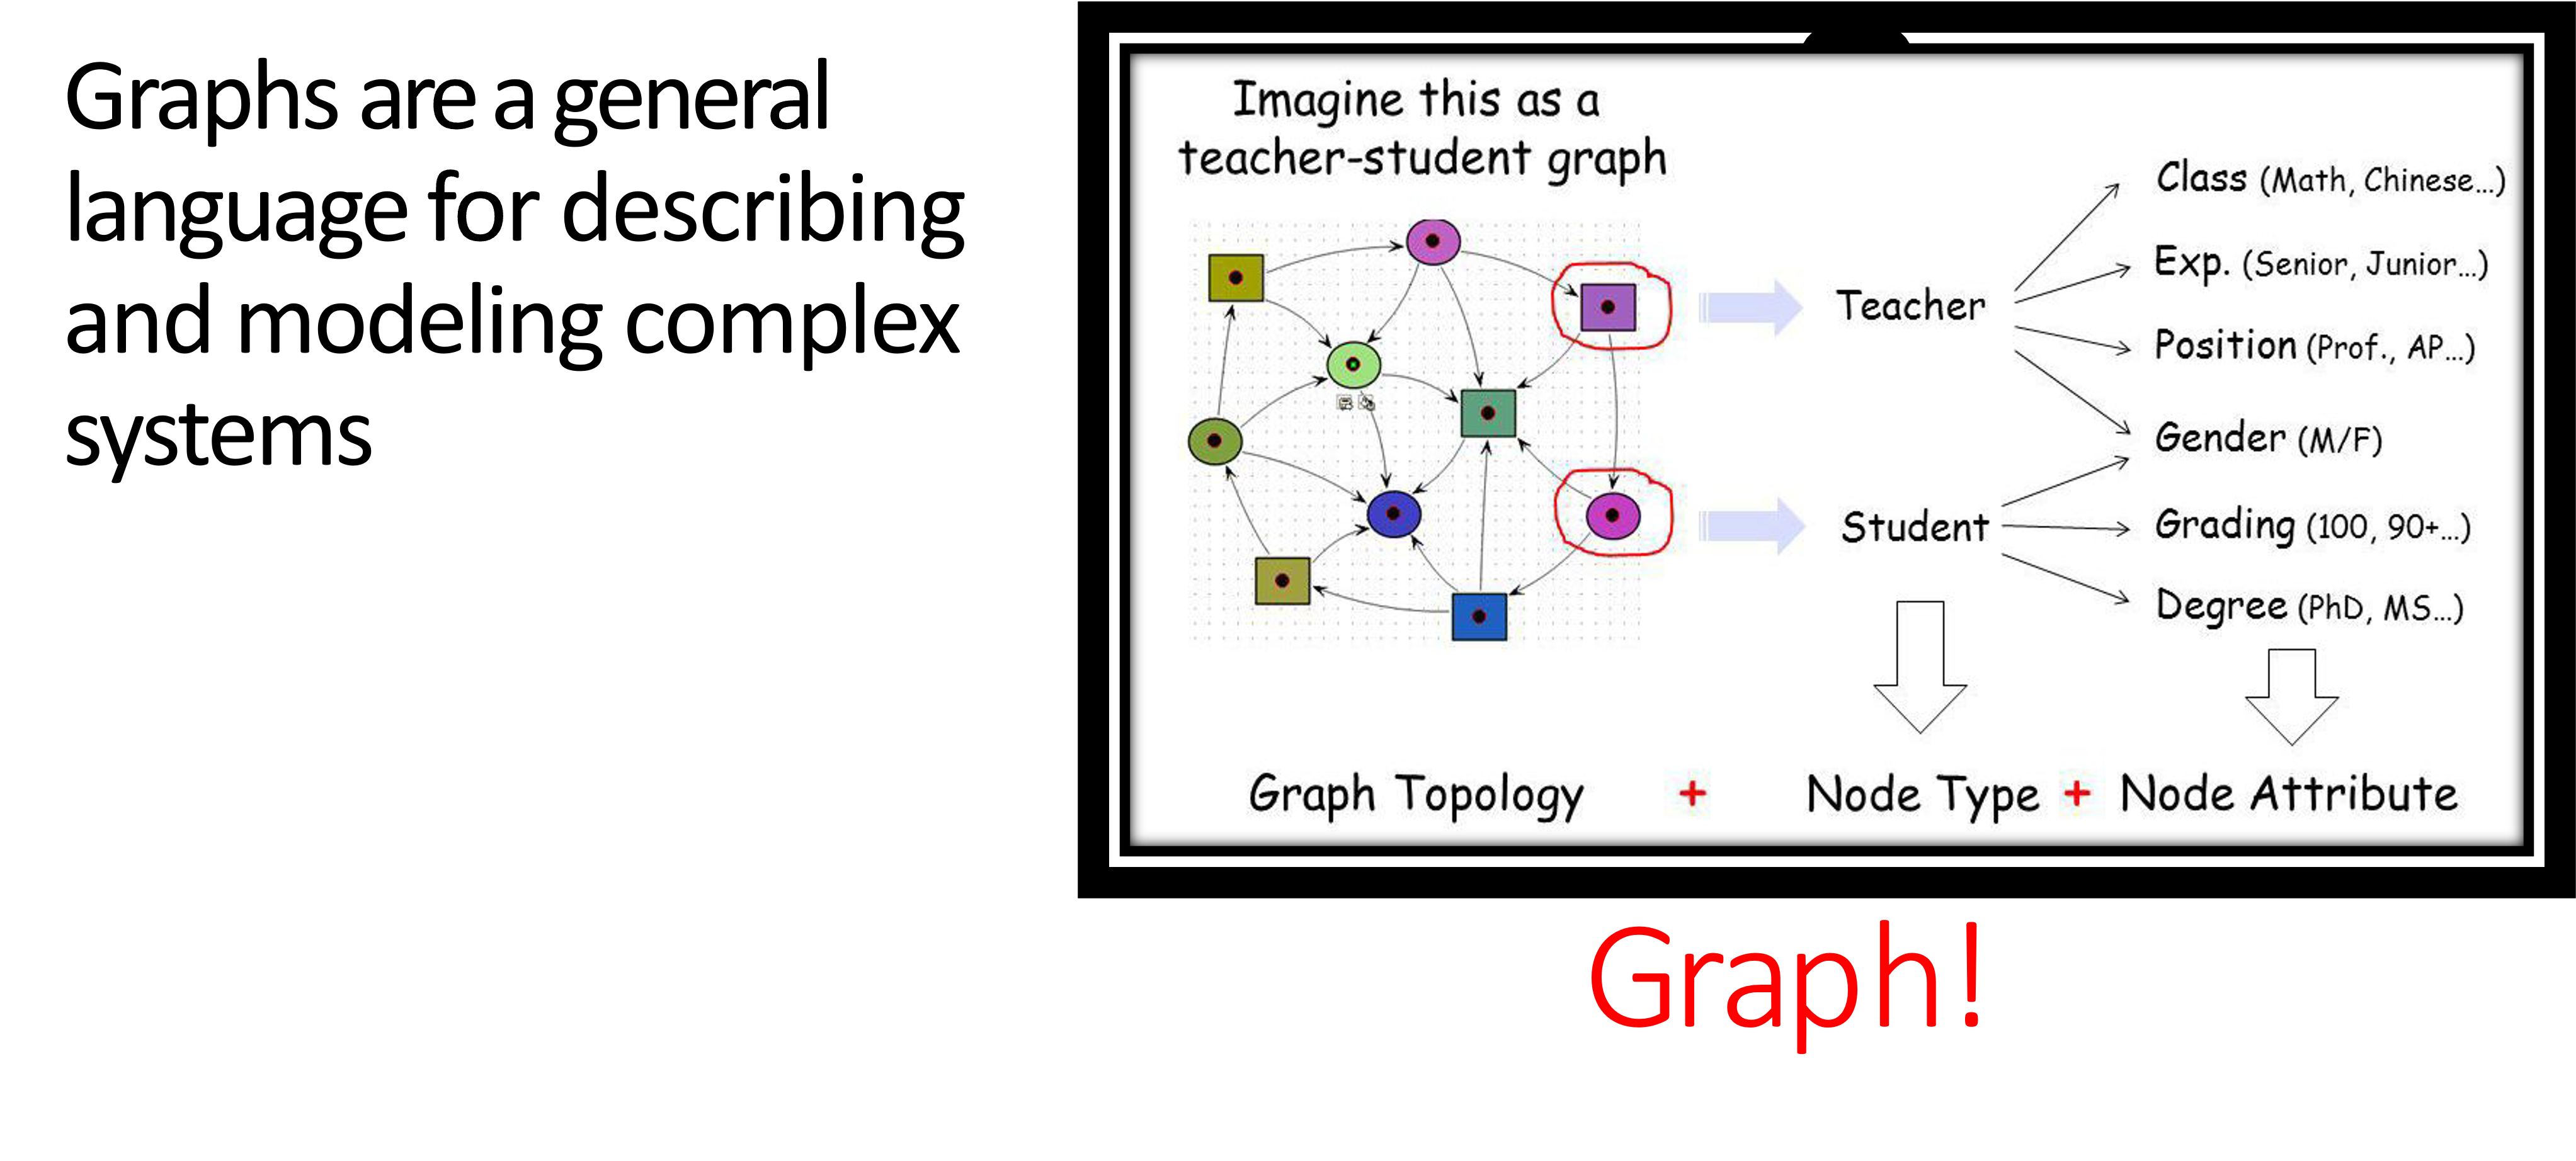
\includegraphics[width=\linewidth,keepaspectratio]{gnn4}
\end{center}	  

\end{frame}


%%%%%%%%%%%%%%%%%%%%%%%%%%%%%%%%%%%%%%%%%%%%%%%%%%%%%%%%%%%
\begin{frame}[fragile]\frametitle{Data as Graphs - Explicit }

\begin{center}
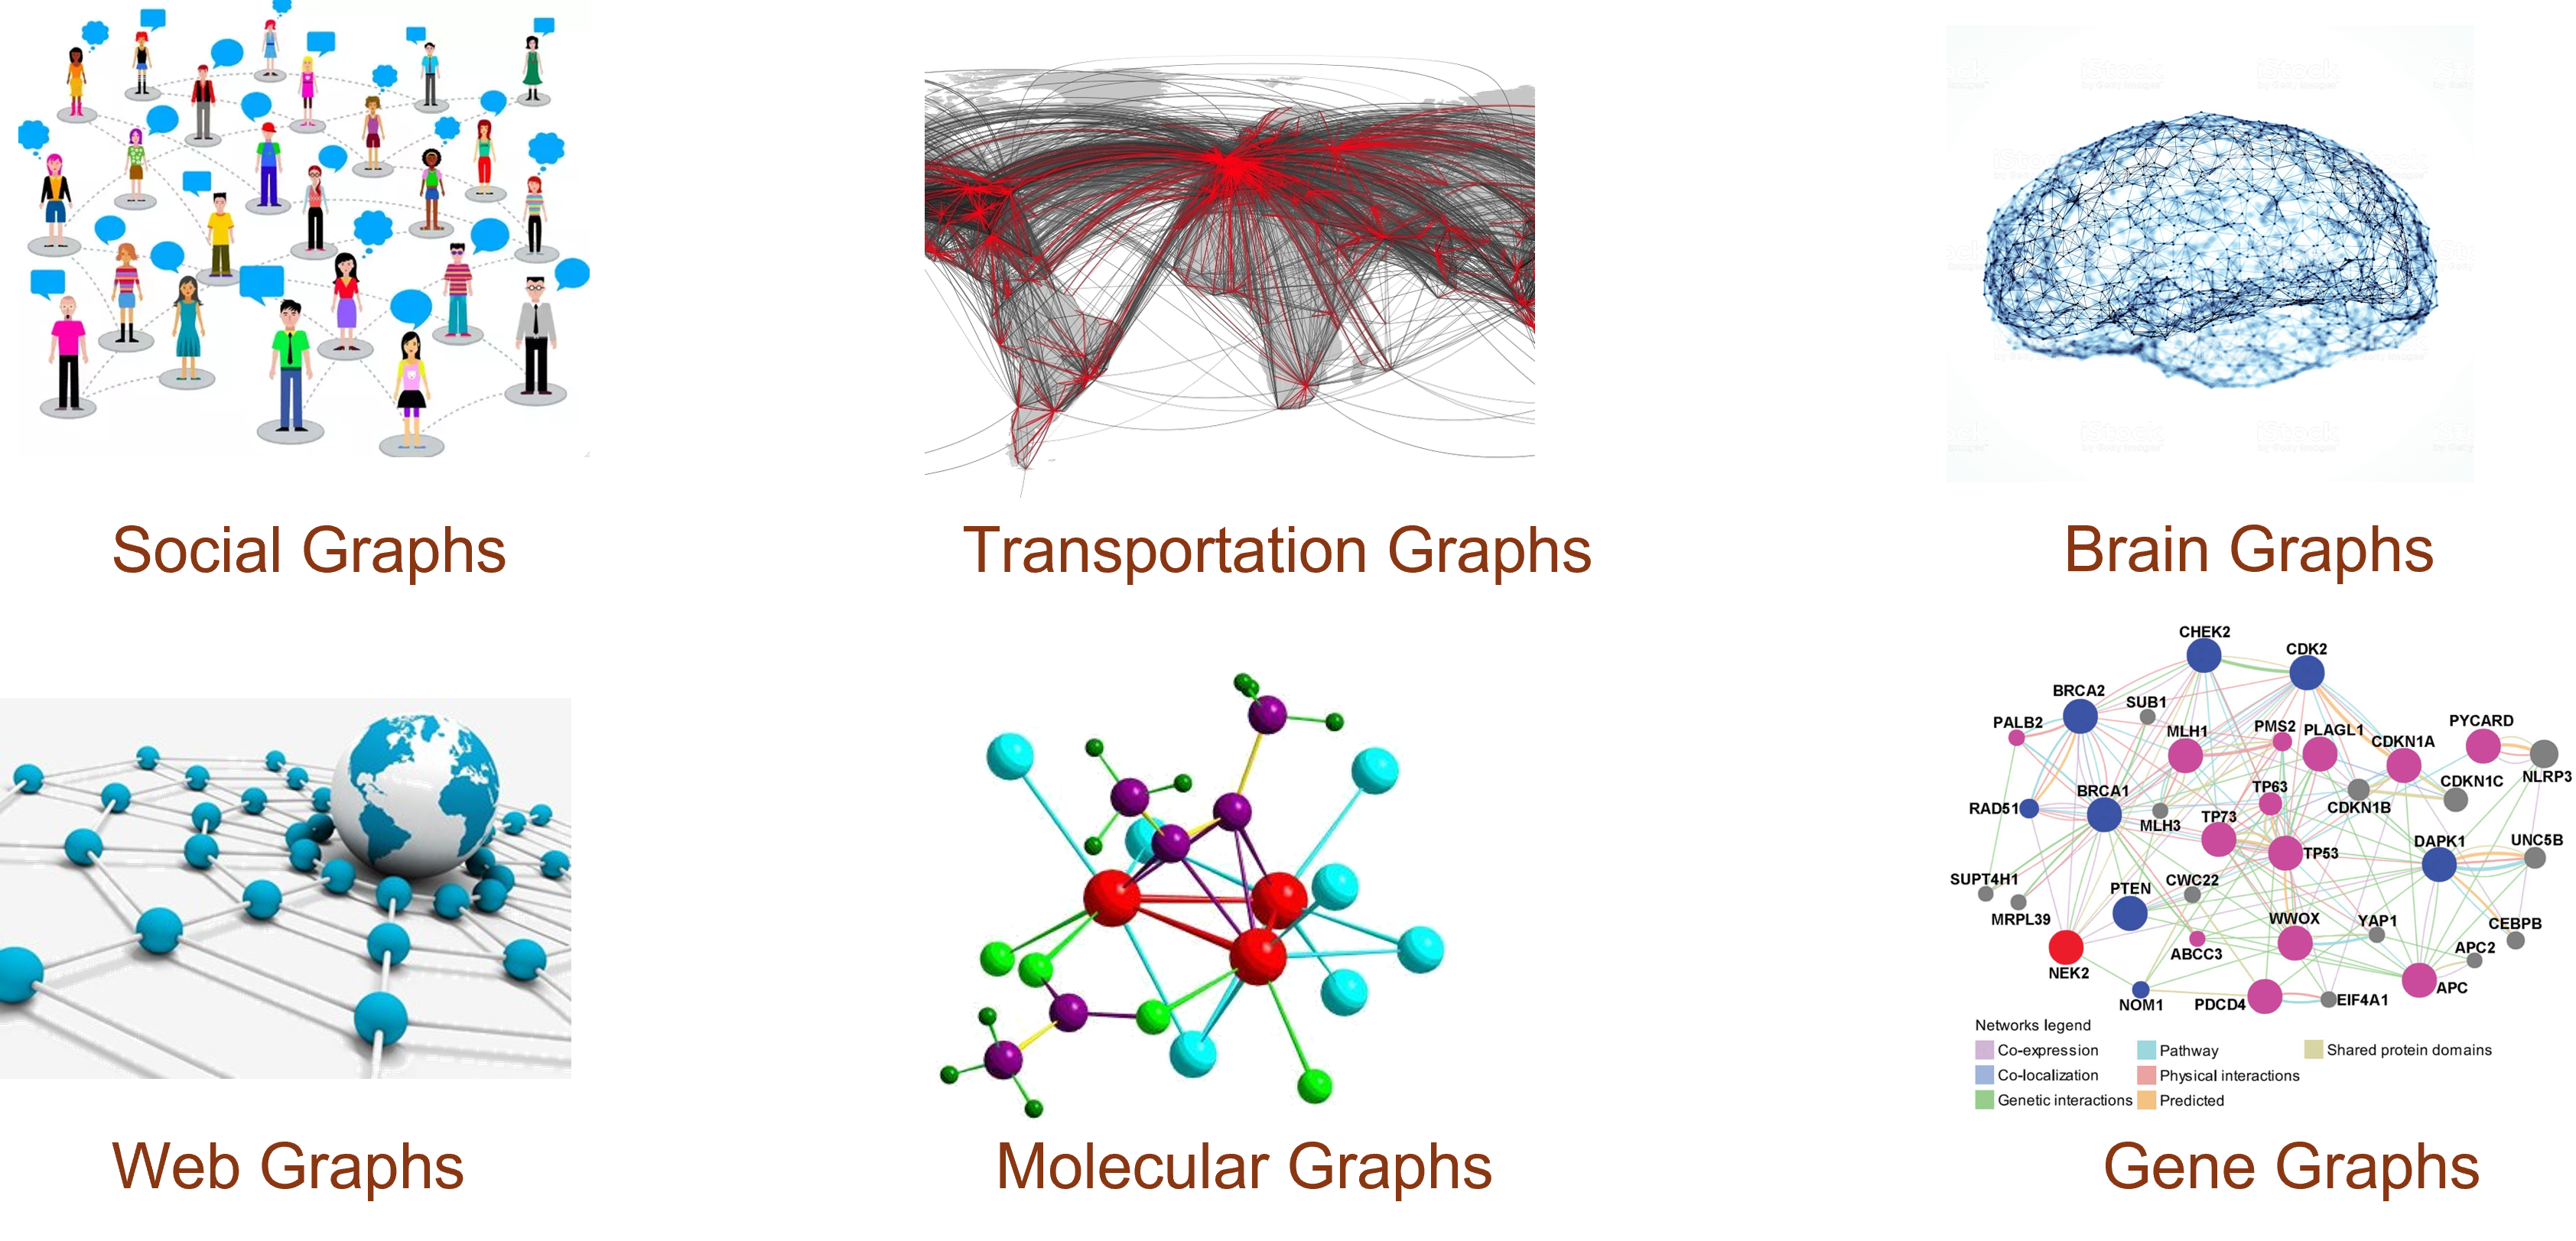
\includegraphics[width=\linewidth,keepaspectratio]{gnn5}
\end{center}	  

\end{frame}

%%%%%%%%%%%%%%%%%%%%%%%%%%%%%%%%%%%%%%%%%%%%%%%%%%%%%%%%%%%
\begin{frame}[fragile]\frametitle{Data as Graphs - Implicit }

\begin{center}
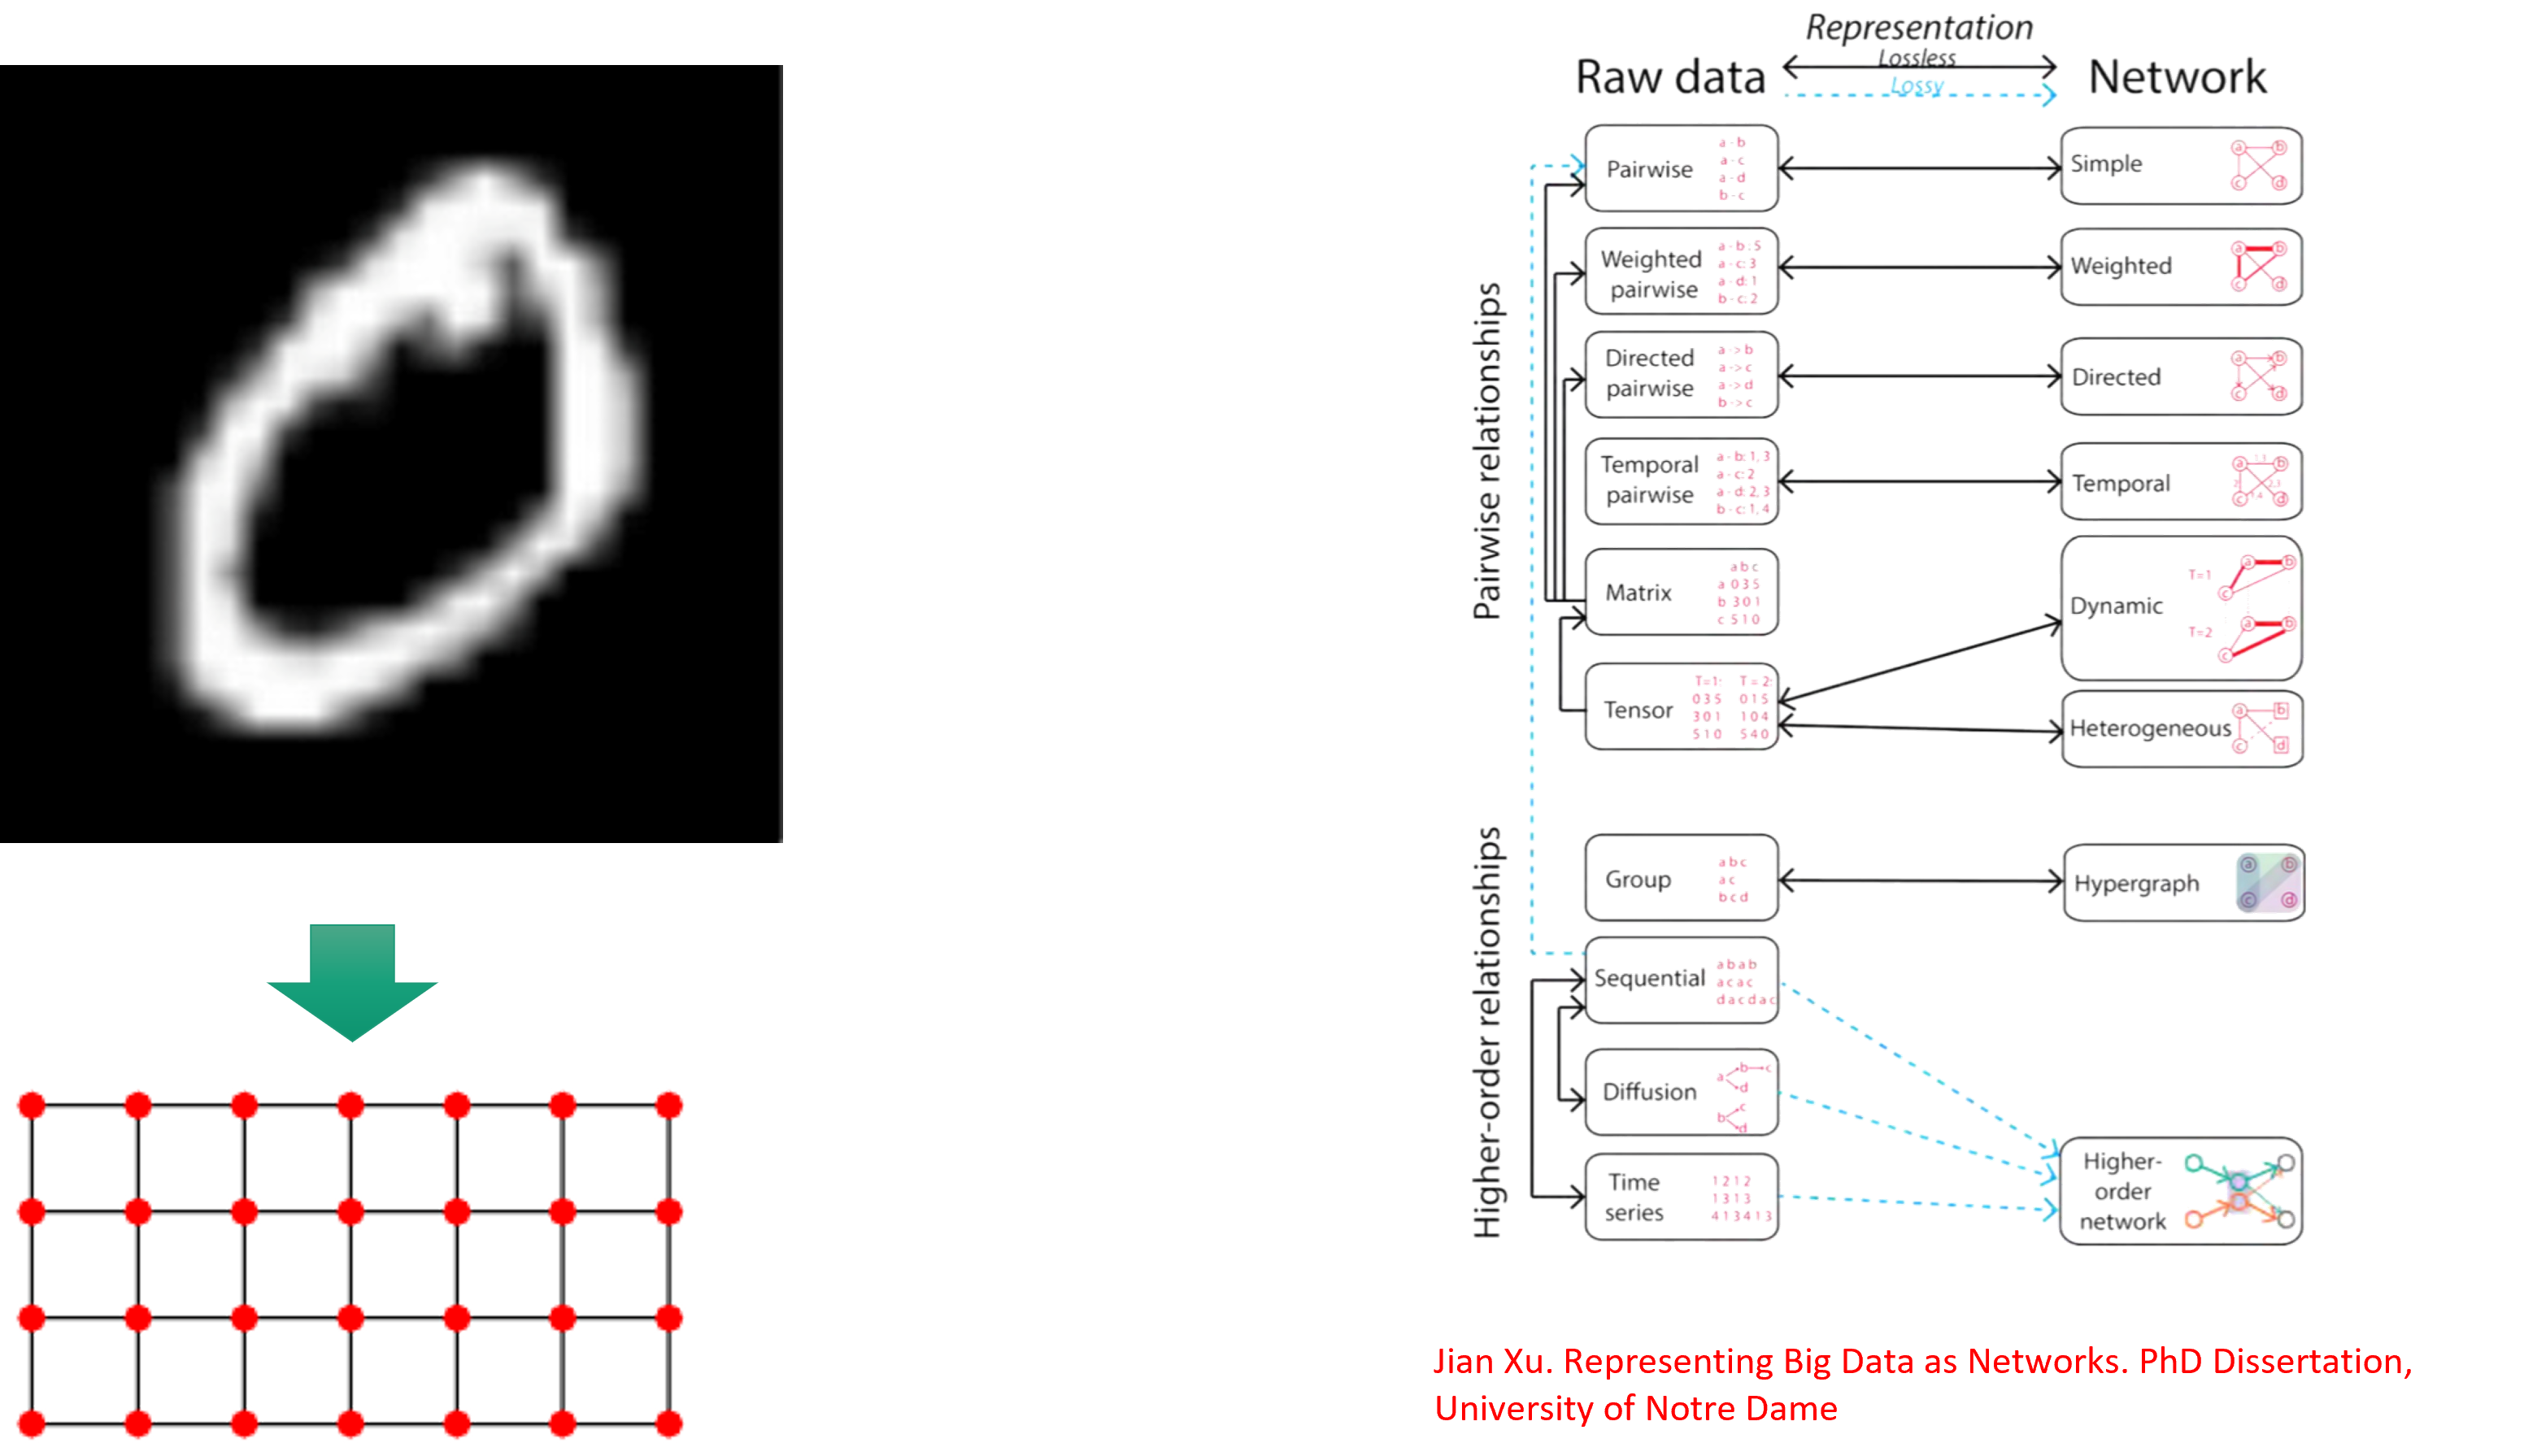
\includegraphics[width=\linewidth,keepaspectratio]{gnn6}
\end{center}	  

\end{frame}



%%%%%%%%%%%%%%%%%%%%%%%%%%%%%%%%%%%%%%%%%%%%%%%%%%%%%%%%%%%
\begin{frame}[fragile]\frametitle{}

\begin{center}
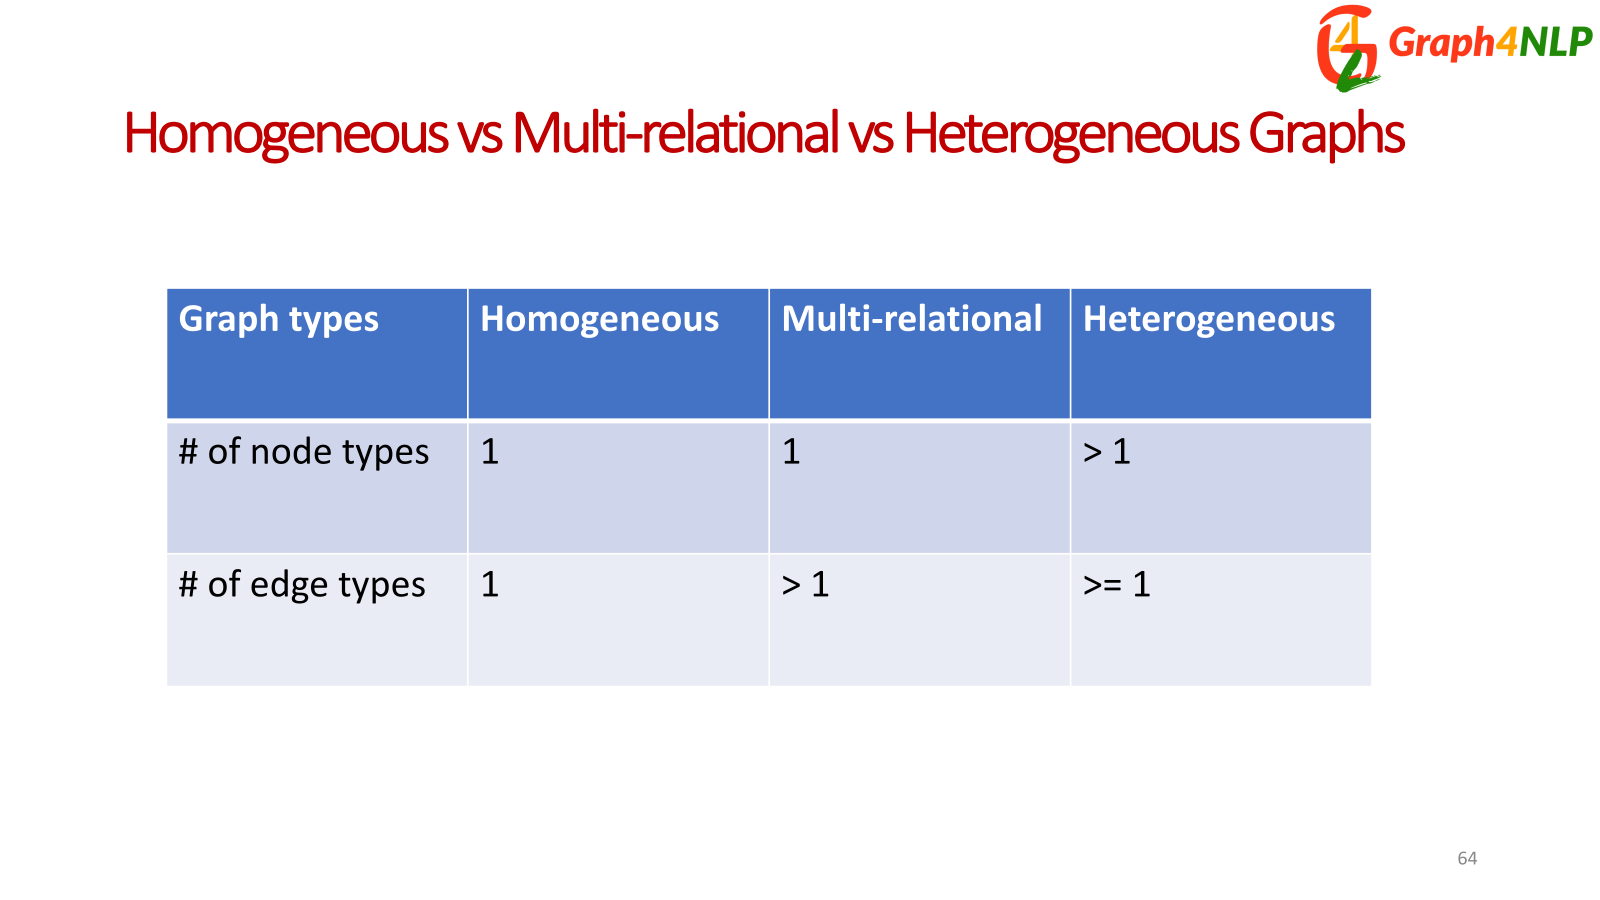
\includegraphics[width=\linewidth,keepaspectratio]{gnn8}
\end{center}	  

\end{frame}

%%%%%%%%%%%%%%%%%%%%%%%%%%%%%%%%%%%%%%%%%%%%%%%%%%%%%%%%%%%%%%%%%%%%%%%%%%%%%%%%%%
\begin{frame}[fragile]\frametitle{Graph Theory Basics}
  \begin{block}{Graph Definition}
    A graph $G$ is an ordered pair $G = (V, E)$, where $V$ is the set of vertices and $E$ is the set of edges connecting the vertices.
  \end{block}
  
  \begin{itemize}
    \item Directed vs. undirected graphs
    \item Nodes (vertices) and relationships (edges)
    \item Properties and labels
  \end{itemize}
\end{frame}

%%%%%%%%%%%%%%%%%%%%%%%%%%%%%%%%%%%%%%%%%%%%%%%%%%%%%%%%%%%%%%%%%%%%%%%%%%%%%%%%%%
\begin{frame}\frametitle{Graph Components}

\begin{itemize}
\item Node (Vertex): A must data element for constructing a graph
\item Relationship (Edge) : Link between two nodes, can have direction and type.
\item Label: Node category/type such as PERSON, ORG, etc. One node can have many types.
\item Properties: Attributes or fields in Nodes or Edges, eg. A node can have Label PERSON and Property such as ``name: Jane''
\end{itemize}



{\tiny (Ref: Introduction to Neo4j - a hands-on crash course - neo4j)}
\end{frame}




%%%%%%%%%%%%%%%%%%%%%%%%%%%%%%%%%%%%%%%%%%%%%%%%%%%%%%%%%%%%%%%%%%%%%%%%%%%%%%%%%%
\begin{frame}\frametitle{Nodes}


\begin{center}
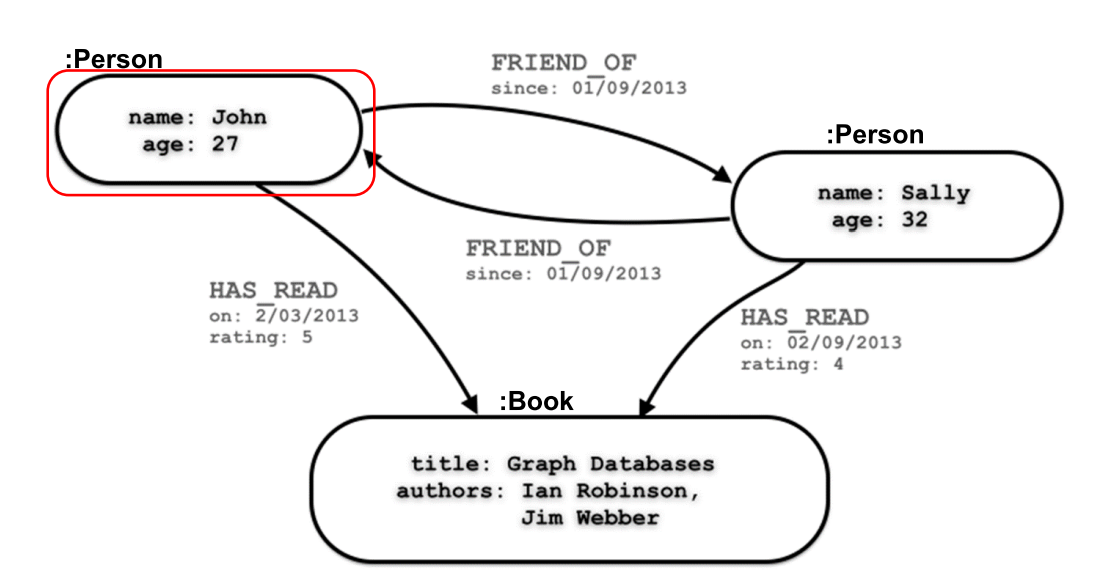
\includegraphics[width=\linewidth,keepaspectratio]{neo4j33}
\end{center}	

{\tiny (Ref: CIS 6930 - Advanced Databases - Neo4j )}
\end{frame}


%%%%%%%%%%%%%%%%%%%%%%%%%%%%%%%%%%%%%%%%%%%%%%%%%%%%%%%%%%%%%%%%%%%%%%%%%%%%%%%%%%
\begin{frame}\frametitle{Relationships}


\begin{center}
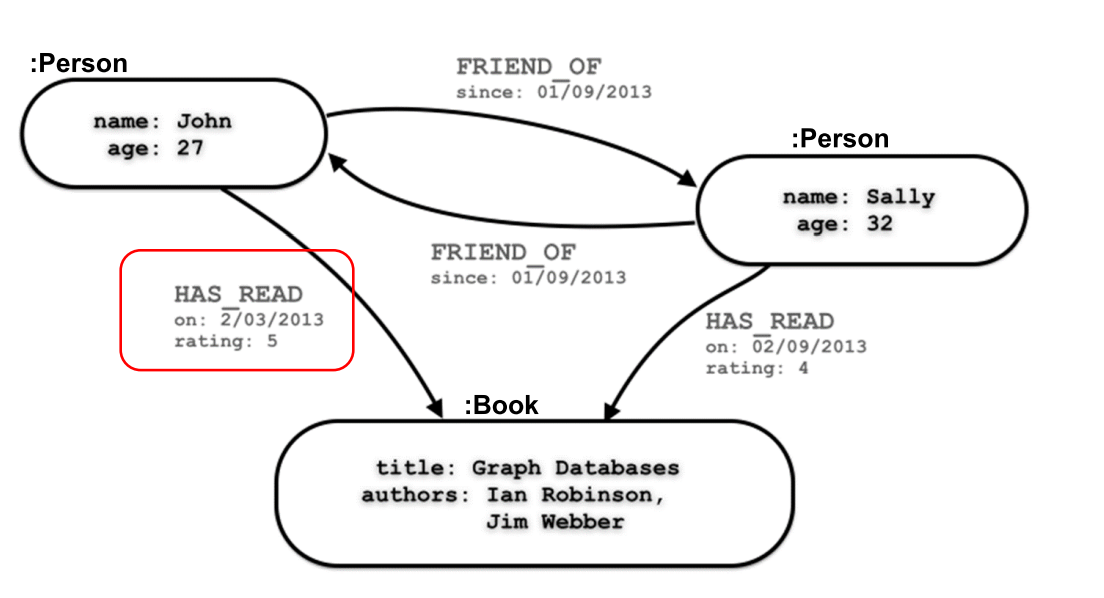
\includegraphics[width=\linewidth,keepaspectratio]{neo4j34}
\end{center}	

{\tiny (Ref: CIS 6930 - Advanced Databases - Neo4j )}
\end{frame}

%%%%%%%%%%%%%%%%%%%%%%%%%%%%%%%%%%%%%%%%%%%%%%%%%%%%%%%%%%%%%%%%%%%%%%%%%%%%%%%%%%
\begin{frame}\frametitle{Properties}


\begin{center}
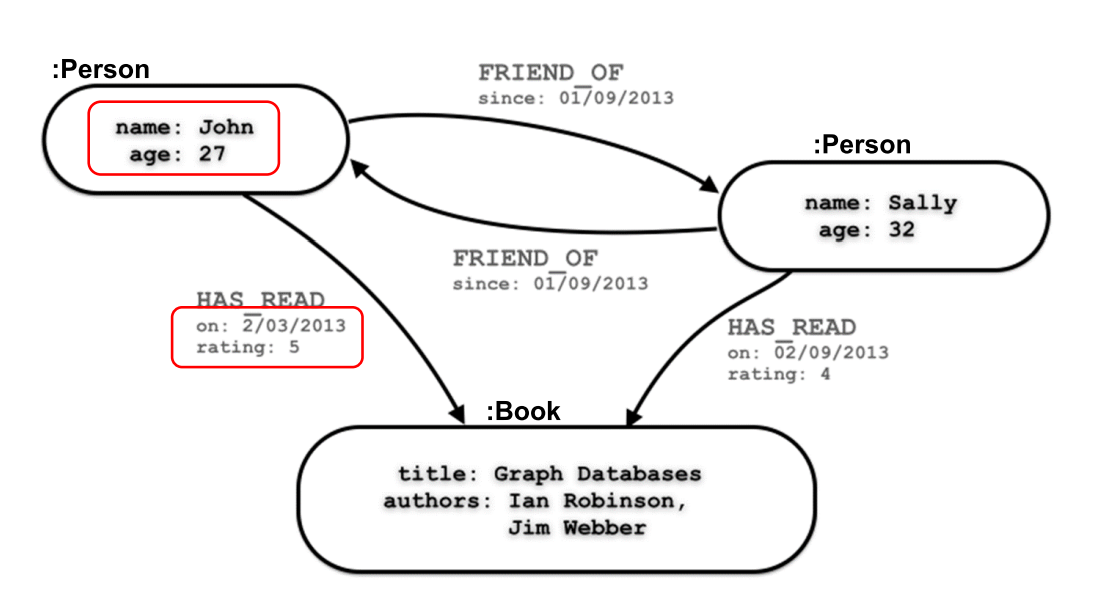
\includegraphics[width=\linewidth,keepaspectratio]{neo4j35}
\end{center}	

{\tiny (Ref: CIS 6930 - Advanced Databases - Neo4j )}
\end{frame}


%%%%%%%%%%%%%%%%%%%%%%%%%%%%%%%%%%%%%%%%%%%%%%%%%%%%%%%%%%%%%%%%%%%%%%%%%%%%%%%%%%
\begin{frame}\frametitle{Labels}


\begin{center}
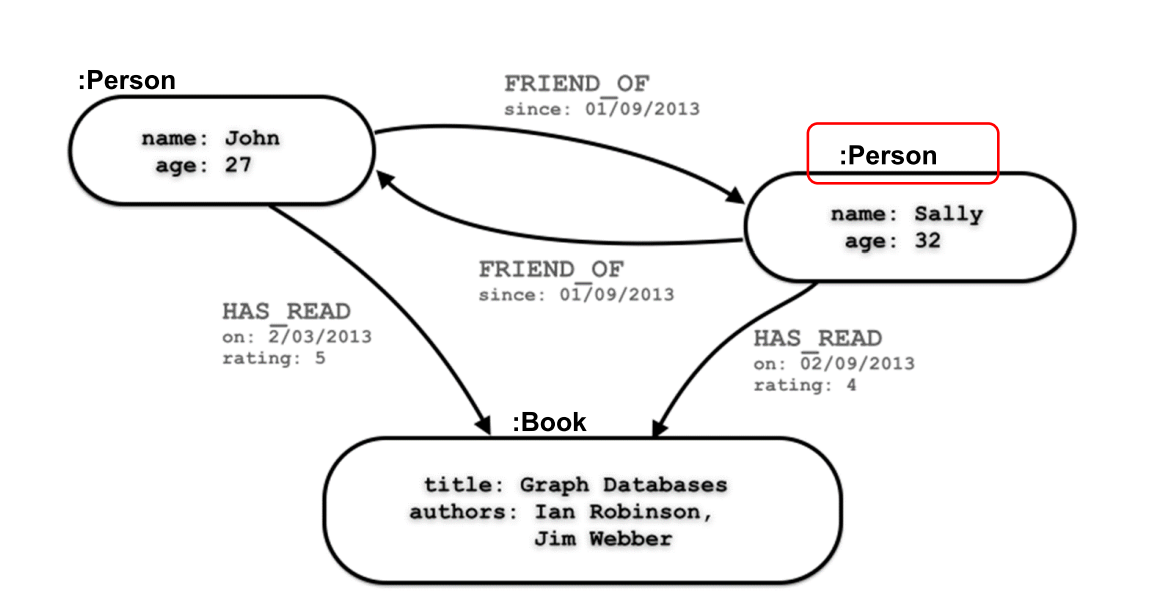
\includegraphics[width=\linewidth,keepaspectratio]{neo4j36}
\end{center}	

{\tiny (Ref: CIS 6930 - Advanced Databases - Neo4j )}
\end{frame}


%%%%%%%%%%%%%%%%%%%%%%%%%%%%%%%%%%%%%%%%%%%%%%%%%%%%%%%%%%%%%%%%%%%%%%%%%%%%%%%%%%
\begin{frame}[fragile]\frametitle{Graph-Edge Types}

\begin{itemize}
\item Undirected graph: edges are bidirectional, e.g. Michale is brother of John, necessarily means that John is brother of Michale.
\item Directed graph: edges have one direction, e.g. A likes B does not necessarily mean that B likes A.
\item Weighted graph: edges have weights, e.g. connection from city A to city B via road R1 will have wright, say, 8, due to high traffic, but via road R2, may have weight 2, due to lower traffic.
\end{itemize}

\end{frame}



% %%%%%%%%%%%%%%%%%%%%%%%%%%%%%%%%%%%%%%%%%%%%%%%%%%%%%%%%%%%%%%%%%%%%%%%%%%%%%%%%%%
% \begin{frame}\frametitle{Summary: Different Kinds of Graphs}

% \begin{center}
% 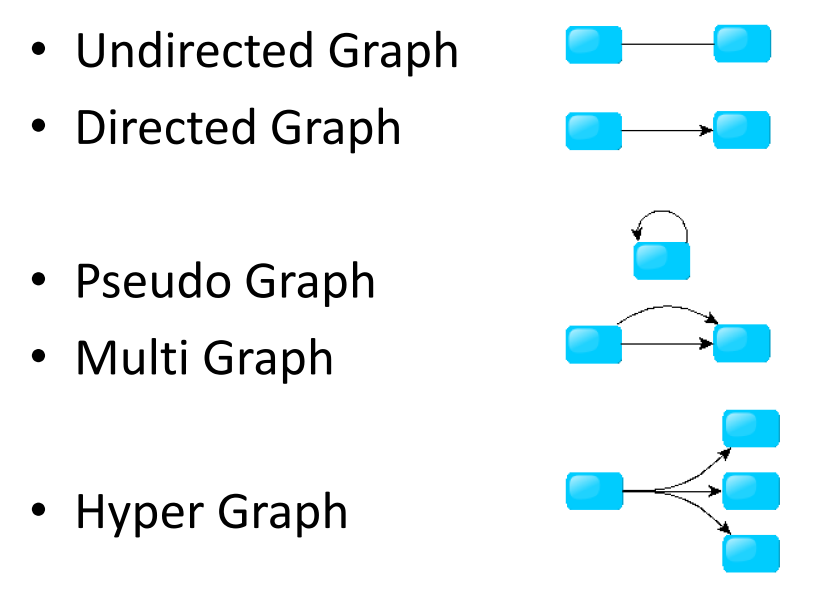
\includegraphics[width=0.5\linewidth,keepaspectratio]{neo4j41}
% \end{center}
 

% {\tiny (Ref: CIntroduction to Graph Databases - Max De Marzi )}
% \end{frame}

% %%%%%%%%%%%%%%%%%%%%%%%%%%%%%%%%%%%%%%%%%%%%%%%%%%%%%%%%%%%%%%%%%%%%%%%%%%%%%%%%%%
% \begin{frame}\frametitle{Summary: More Kinds of Graphs}

% \begin{center}
% 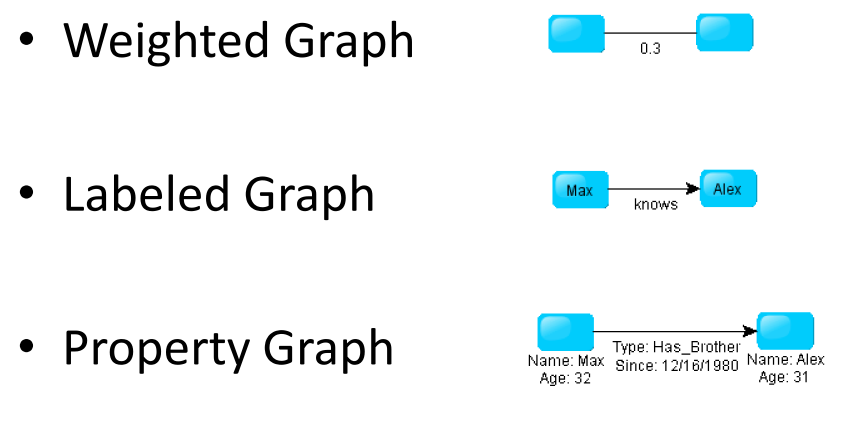
\includegraphics[width=0.5\linewidth,keepaspectratio]{neo4j42}
% \end{center}
 

% {\tiny (Ref: CIntroduction to Graph Databases - Max De Marzi )}
% \end{frame}


% %%%%%%%%%%%%%%%%%%%%%%%%%%%%%%%%%%%%%%%%%%%%%%%%%%%%%%%%%%%
% \begin{frame}[fragile]\frametitle{Graphs and features}

% \begin{center}
% 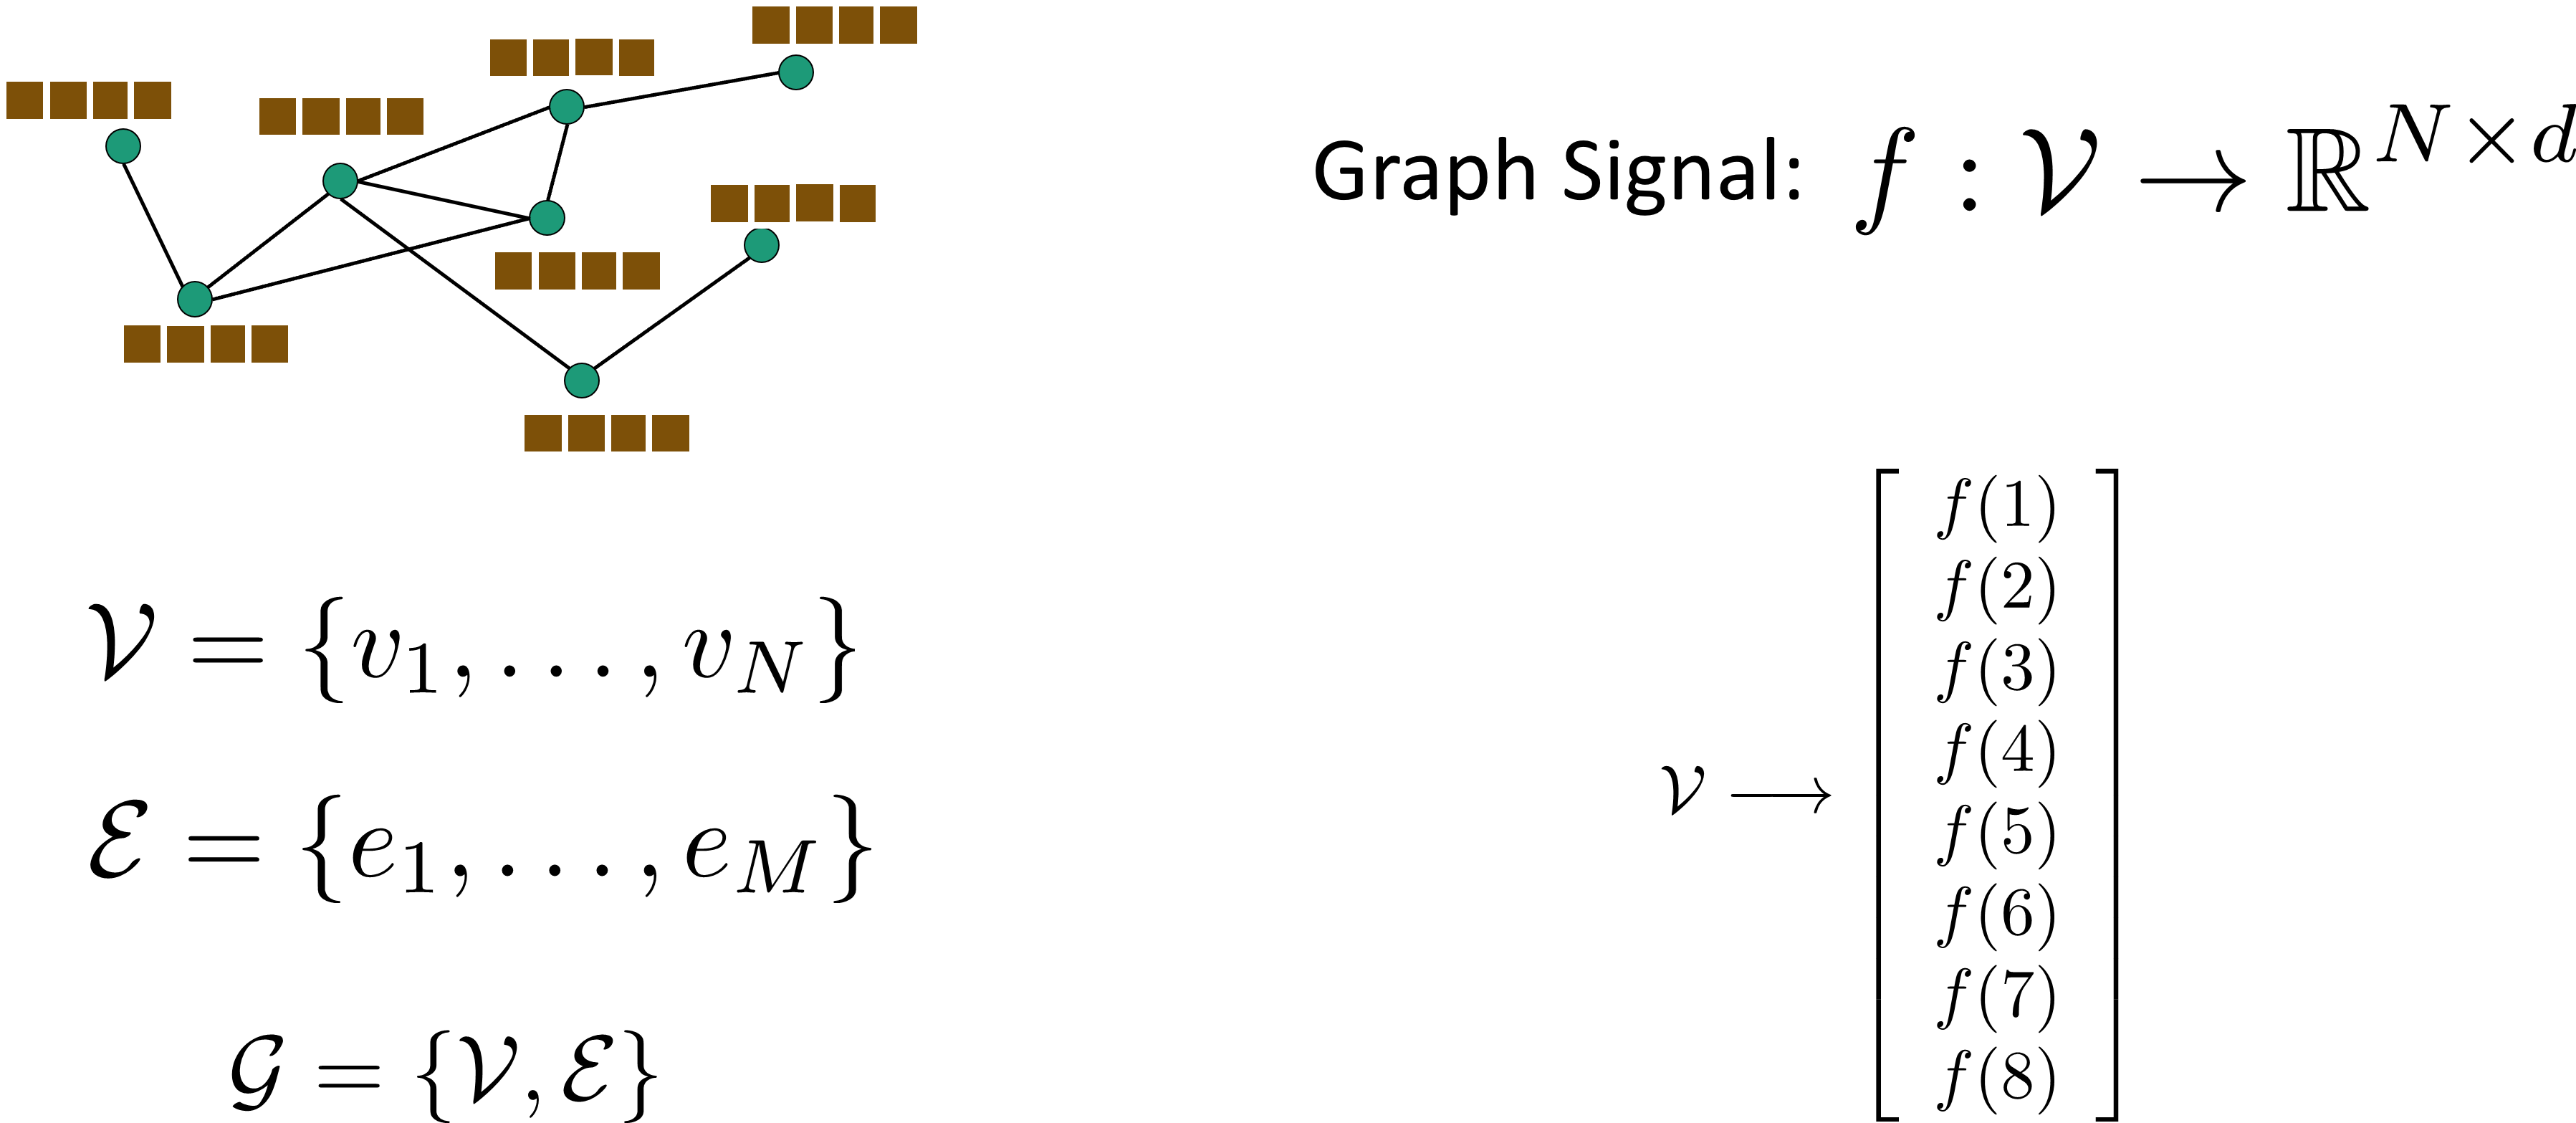
\includegraphics[width=\linewidth,keepaspectratio]{gnn9}
% \end{center}	  

% \end{frame}

% %%%%%%%%%%%%%%%%%%%%%%%%%%%%%%%%%%%%%%%%%%%%%%%%%%%%%%%%%%%
% \begin{frame}[fragile]\frametitle{Matrix Representations of Graphs}

% \begin{center}
% 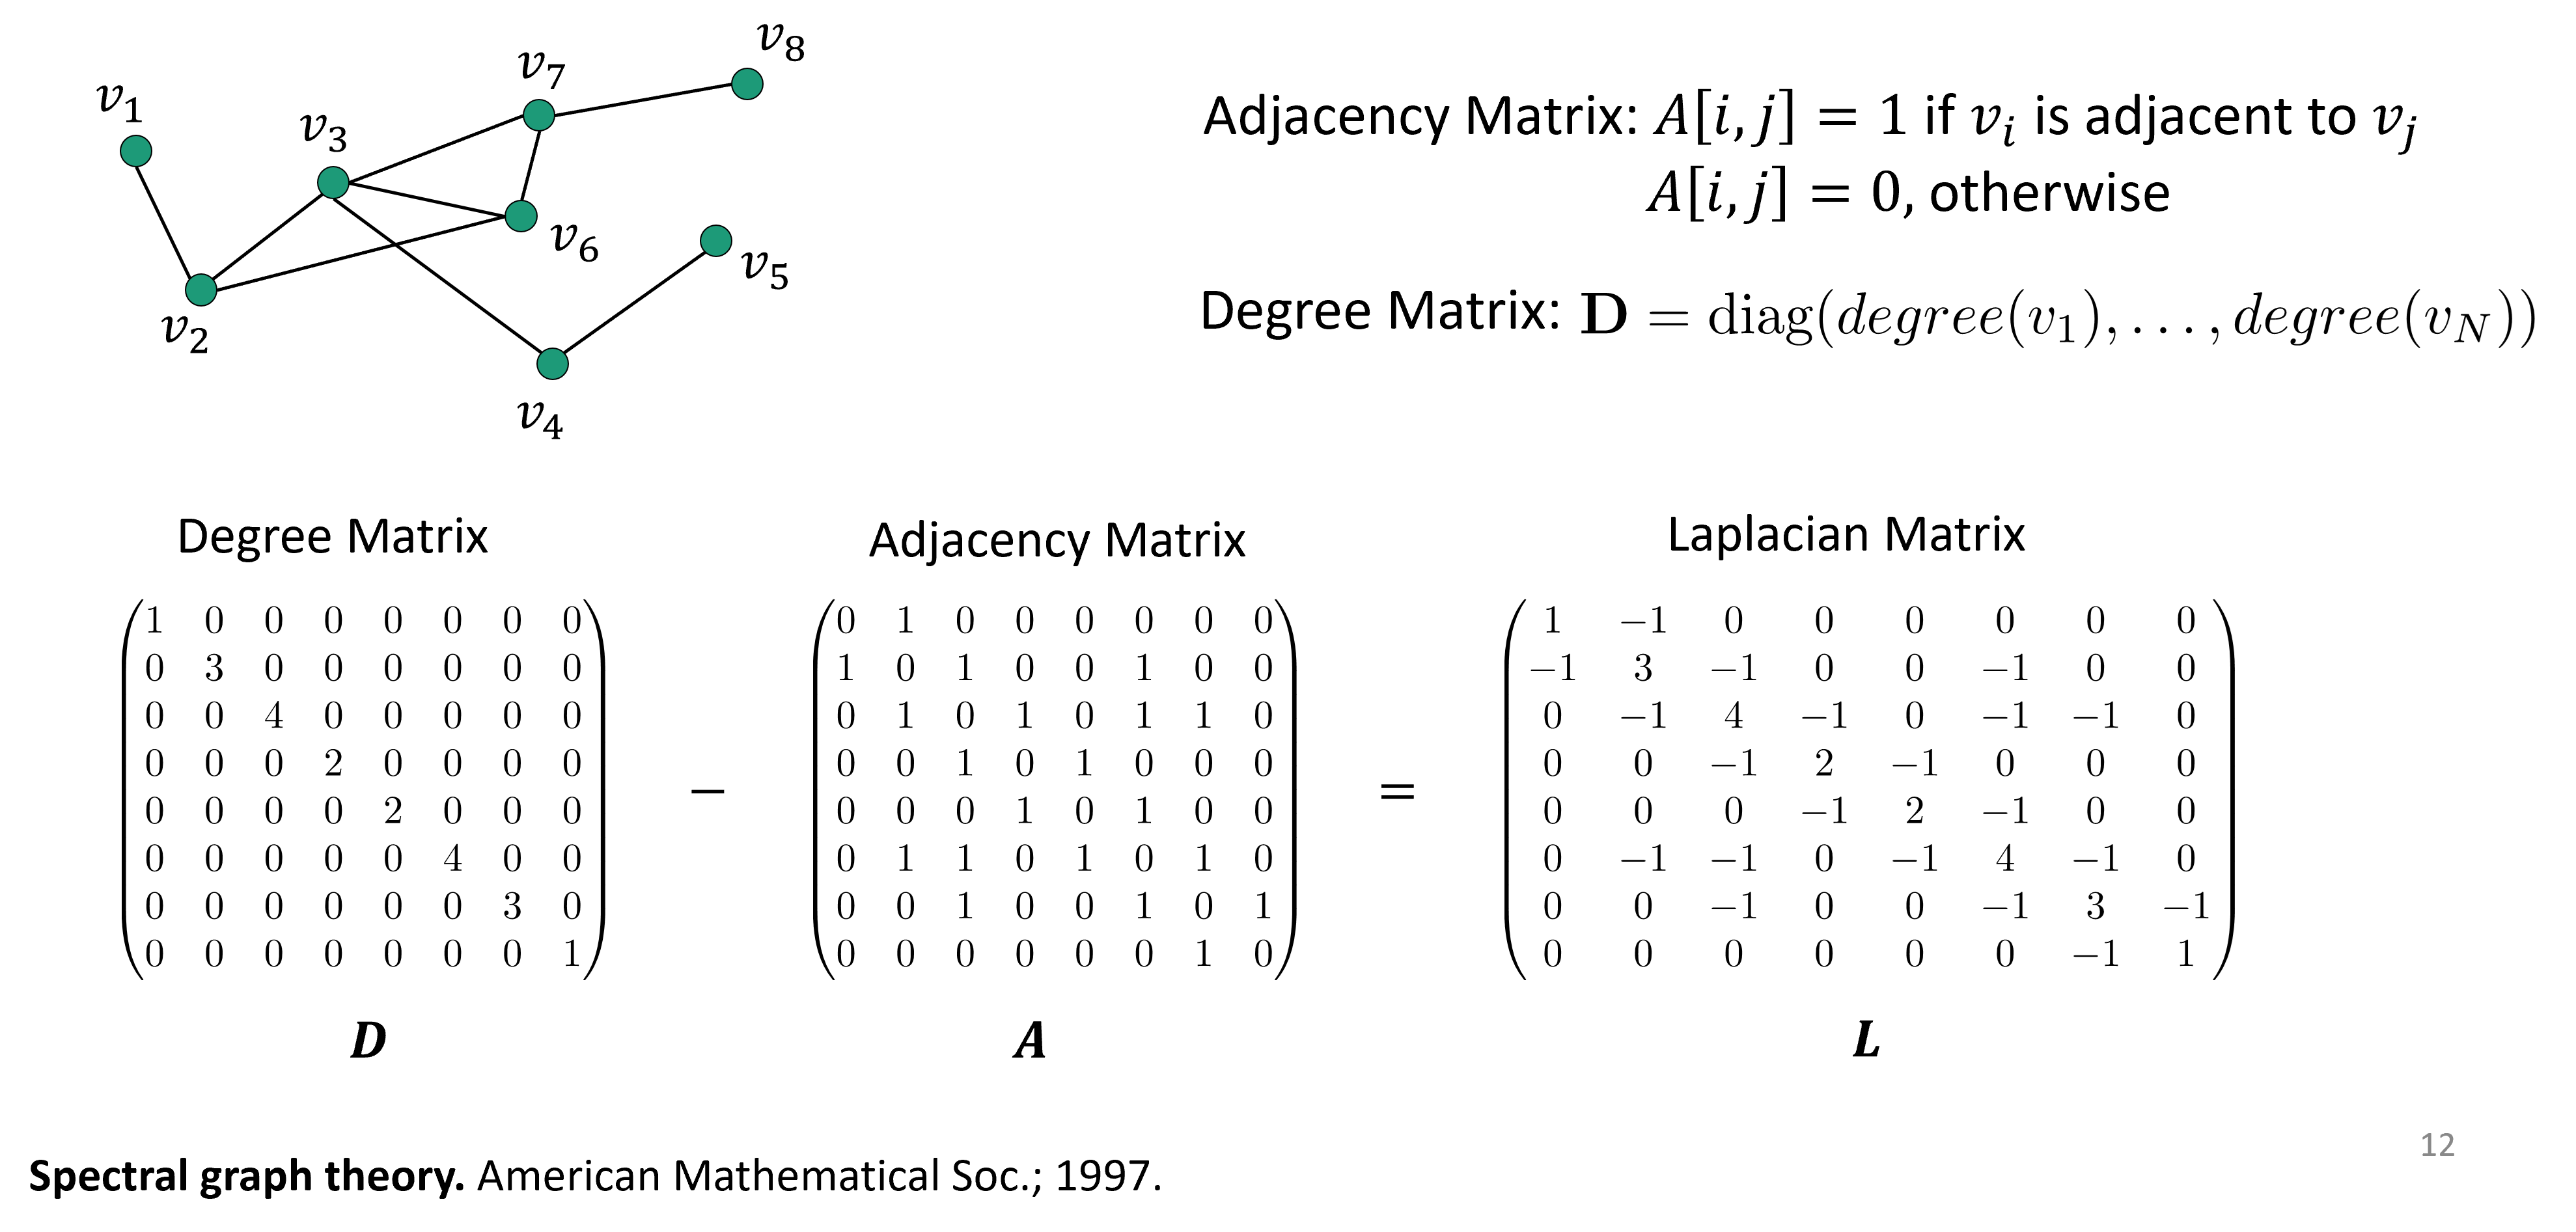
\includegraphics[width=\linewidth,keepaspectratio]{gnn10}
% \end{center}	  

% \end{frame}

%%%%%%%%%%%%%%%%%%%%%%%%%%%%%%%%%%%%%%%%%%%%%%%%%%%%%%%%%%%%%%%%%%%%%%%%%%%%%%%%%%
\begin{frame}[fragile]\frametitle{Graph Algorithms}
  \begin{itemize}
    \item Graph algorithms are a set of computational techniques for analyzing and processing graphs.
    \item Some popular graph algorithms include:
    \begin{itemize}
      \item Breadth-First Search (BFS)
      \item Depth-First Search (DFS)
      \item Shortest Path Algorithms (Dijkstra's, Bellman-Ford)
      \item Clustering Algorithms (Louvain, Label Propagation)
      \item PageRank, Betweenness Centrality, and more.
    \end{itemize}
    \item These algorithms are fundamental building blocks for solving a wide range of problems.
  \end{itemize}
\end{frame}


% %%%%%%%%%%%%%%%%%%%%%%%%%%%%%%%%%%%%%%%%%%%%%%%%%%%%%%%%%%%%%%%%%%%%%%%%%%%%%%%%%%
% \begin{frame}\frametitle{Shortest Path}

% \begin{itemize}
% \item Find shortest path in a weighted graph, to save logistic costs
% \item Dijkstra's or A* algorithm
% \item Graph Traversals: can edges be traversed multiple times or nodes traversed multiple times? Neo4j prefers not to traverse edges multiple times, thus making it fast.
% \end{itemize}

% Application: :
% \begin{center}
% 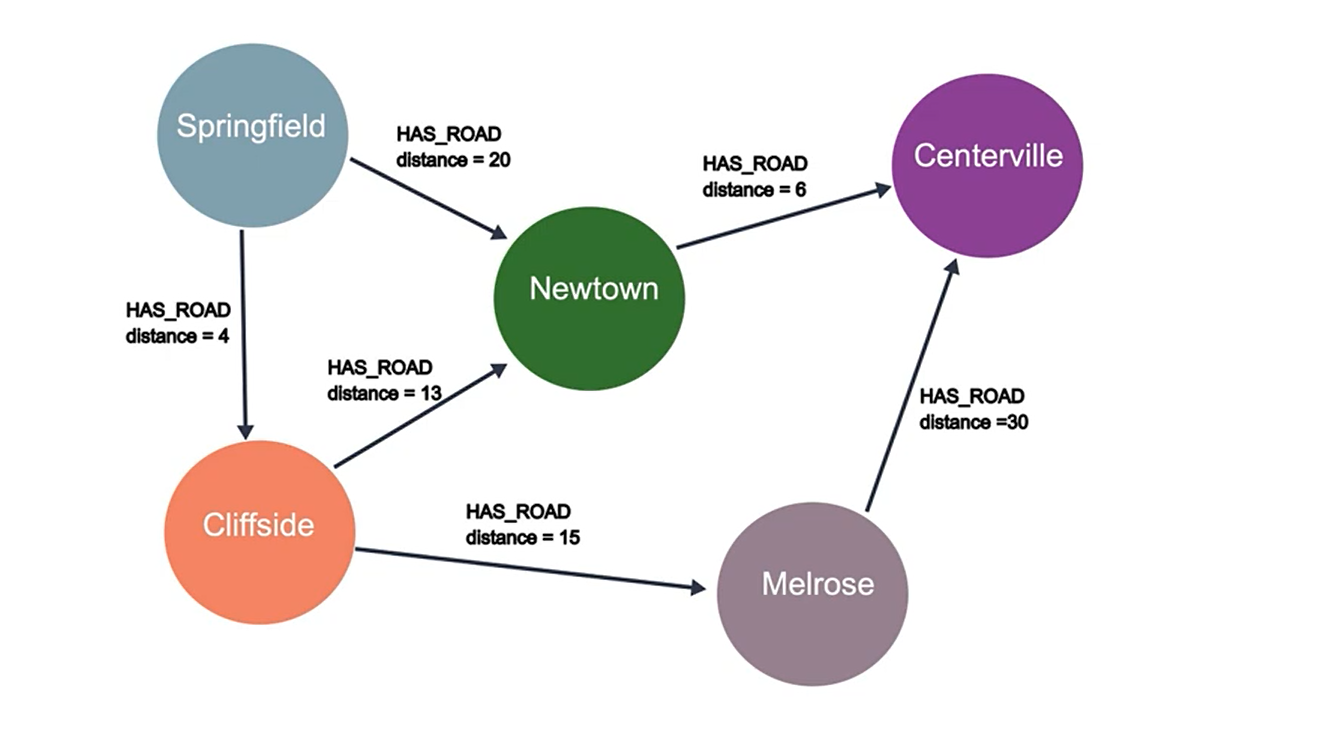
\includegraphics[width=0.6\linewidth,keepaspectratio]{neo4j55}
% \end{center}	

% How many unique paths are there from Springfield to CenterVille?

% {\tiny (Ref: Introduction to Neo4j - a hands-on crash course - neo4j)}
% \end{frame}

%%%%%%%%%%%%%%%%%%%%%%%%%%%%%%%%%%%%%%%%%%%%%%%%%%%%%%%%%%%
\begin{frame}[fragile]\frametitle{Why Graphs? Why Now?}

\begin{itemize}
\item Universal language for describing complex data: Networks/graphs from science, nature, and technology are more similar than one would expect
\item Shared vocabulary between fields: Computer Science, Social science, Physics, Biology, Economics 
\item Data availability (+ computational challenges): Social/Internet, text, logic, program, bio, health, and medical
\item Impact: Social networking, Social media, Drug design, Event detection, Natural language processing, Computer vision, and Logic reasoning
\end{itemize}

\end{frame}

% %%%%%%%%%%%%%%%%%%%%%%%%%%%%%%%%%%%%%%%%%%%%%%%%%%%%%%%%%%%
% \begin{frame}[fragile]\frametitle{Graph Analytics Workflow}
  % \begin{itemize}
    % \item Define the problem: Identify the business problem that can be solved using graph analytics.
    % \item Data modeling: Create a graph data model that represents the problem domain.
    % \item Data import: Import data into the graph database.
    % \item Algorithm selection: Choose the appropriate graph algorithm(s) for the problem at hand.
    % \item Algorithm execution: Run the selected algorithm(s) on the graph data.
    % \item Result interpretation: Analyze and interpret the algorithm output to gain insights.
  % \end{itemize}
% \end{frame}

% %%%%%%%%%%%%%%%%%%%%%%%%%%%%%%%%%%%%%%%%%%%%%%%%%%%%%%%%%%%%%%%%%%%%%%%%%%%%%%%%%%
% \begin{frame}\frametitle{Identifying good Graph scenarios - 1/4}

% Does the problem involve understanding relationships between entities?

% Behavioral analysis:

% \begin{center}
% 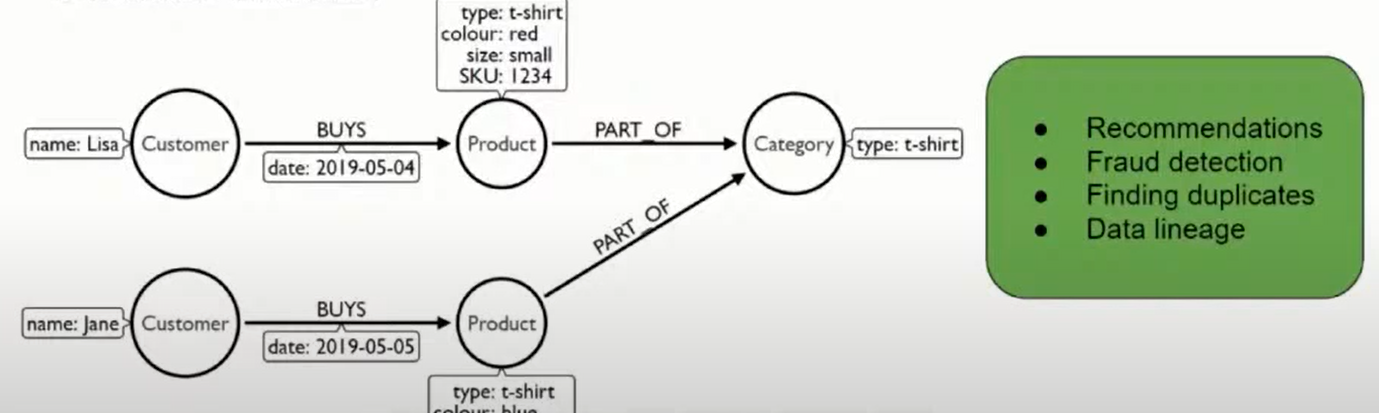
\includegraphics[width=\linewidth,keepaspectratio]{neo4j5}
% \end{center}	  

% {\tiny (Ref: Introduction to Neo4j - a hands-on crash course - neo4j)}
% \end{frame}

% %%%%%%%%%%%%%%%%%%%%%%%%%%%%%%%%%%%%%%%%%%%%%%%%%%%%%%%%%%%%%%%%%%%%%%%%%%%%%%%%%%
% \begin{frame}\frametitle{Identifying good Graph scenarios - 2/4}

% Does the problem involve a lot of self-referencing to the same type of entity?

% Org chart of employees:

% \begin{center}
% 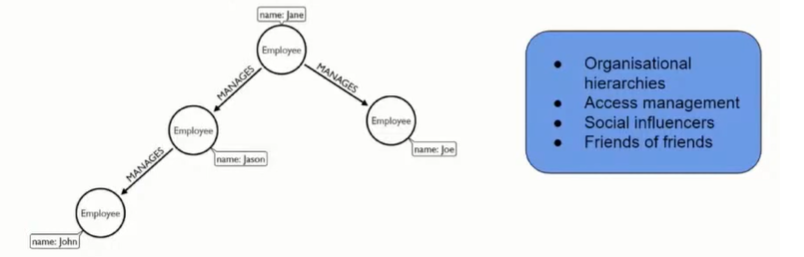
\includegraphics[width=\linewidth,keepaspectratio]{neo4j6}
% \end{center}	  

% {\tiny (Ref: Introduction to Neo4j - a hands-on crash course - neo4j)}
% \end{frame}

% %%%%%%%%%%%%%%%%%%%%%%%%%%%%%%%%%%%%%%%%%%%%%%%%%%%%%%%%%%%%%%%%%%%%%%%%%%%%%%%%%%
% \begin{frame}\frametitle{Identifying good Graph scenarios - 3/4}

% Does the problem explore relationships of varying and unknown depth?

% Changes in manufacturing process:

% \begin{center}
% 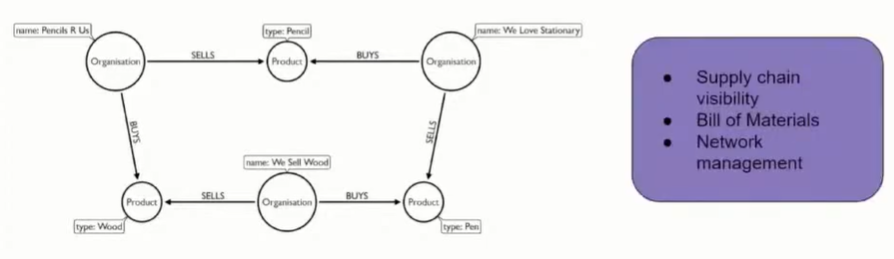
\includegraphics[width=\linewidth,keepaspectratio]{neo4j7}
% \end{center}	  

% {\tiny (Ref: Introduction to Neo4j - a hands-on crash course - neo4j)}
% \end{frame}

% %%%%%%%%%%%%%%%%%%%%%%%%%%%%%%%%%%%%%%%%%%%%%%%%%%%%%%%%%%%%%%%%%%%%%%%%%%%%%%%%%%
% \begin{frame}[fragile]\frametitle{Identifying good Graph scenarios - 4/4}

% Does the problem involve discovering lots of different routes or paths?

% Optimum logistics:

% \begin{center}
% 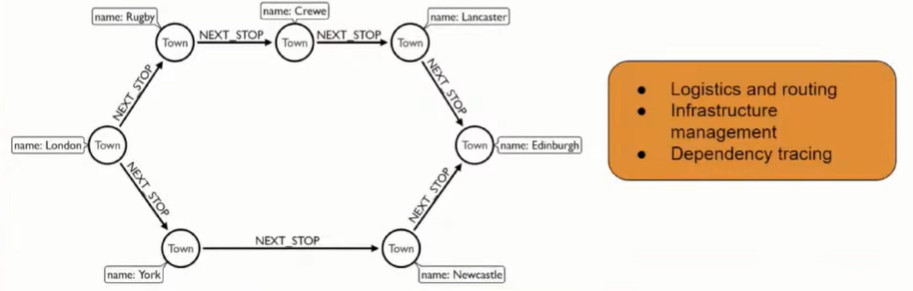
\includegraphics[width=\linewidth,keepaspectratio]{neo4j8}
% \end{center}	  

% {\tiny (Ref: Introduction to Neo4j - a hands-on crash course - neo4j)}
% \end{frame}

\section[Db]{Graph Database}
%%%%%%%%%%%%%%%%%%%%%%%%%%%%%%%%%%%%%%%%%%%%%%%%%%%%%%%%%%%%%%%%%%%%%%%%%%%%%%%%%%
\begin{frame}[fragile]\frametitle{}
\begin{center}
{\Large Graph Database}
\end{center}
\end{frame}

%%%%%%%%%%%%%%%%%%%%%%%%%%%%%%%%%%%%%%%%%%%%%%%%%%%%%%%%%%%
\begin{frame}[fragile]\frametitle{Why?}

Graph databases keep data in its natural, connected state.

\begin{center}
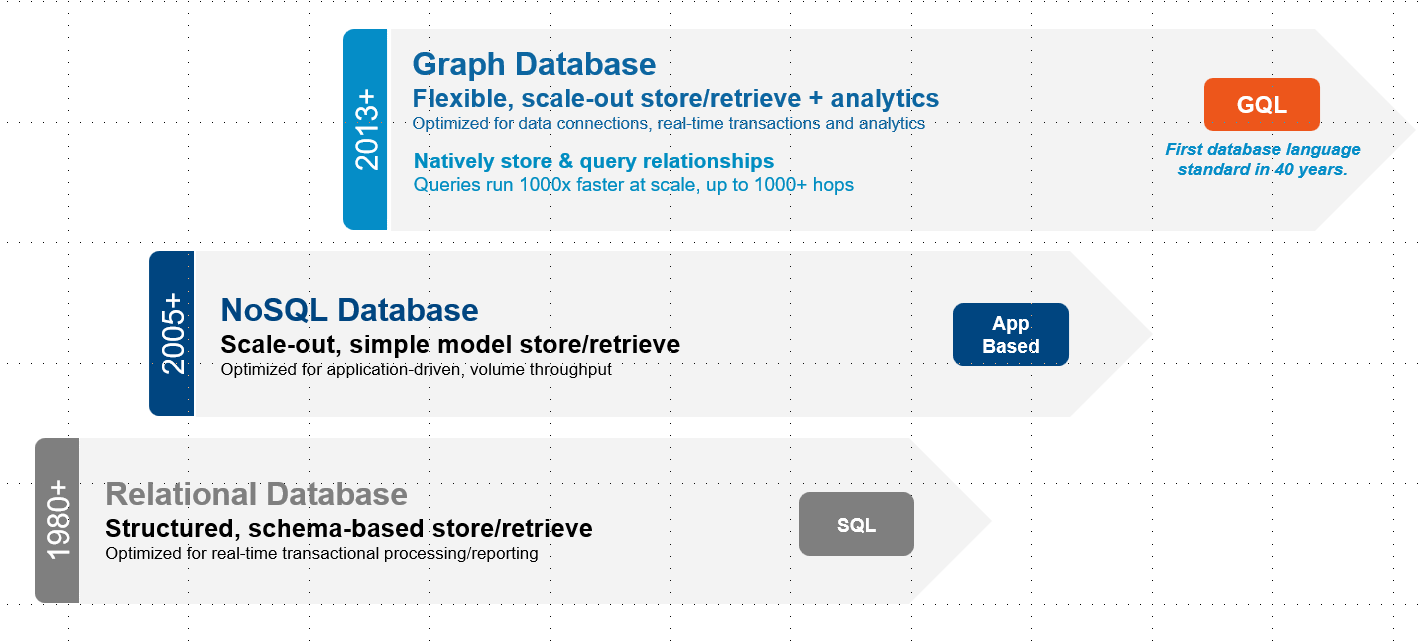
\includegraphics[width=\linewidth,keepaspectratio]{neo4j107}
\end{center}	  

\end{frame}

%%%%%%%%%%%%%%%%%%%%%%%%%%%%%%%%%%%%%%%%%%%%%%%%%%%%%%%%%%%%%%%%%%%%%%%%%%%%%%%%%%
\begin{frame}[fragile]\frametitle{}

\begin{center}
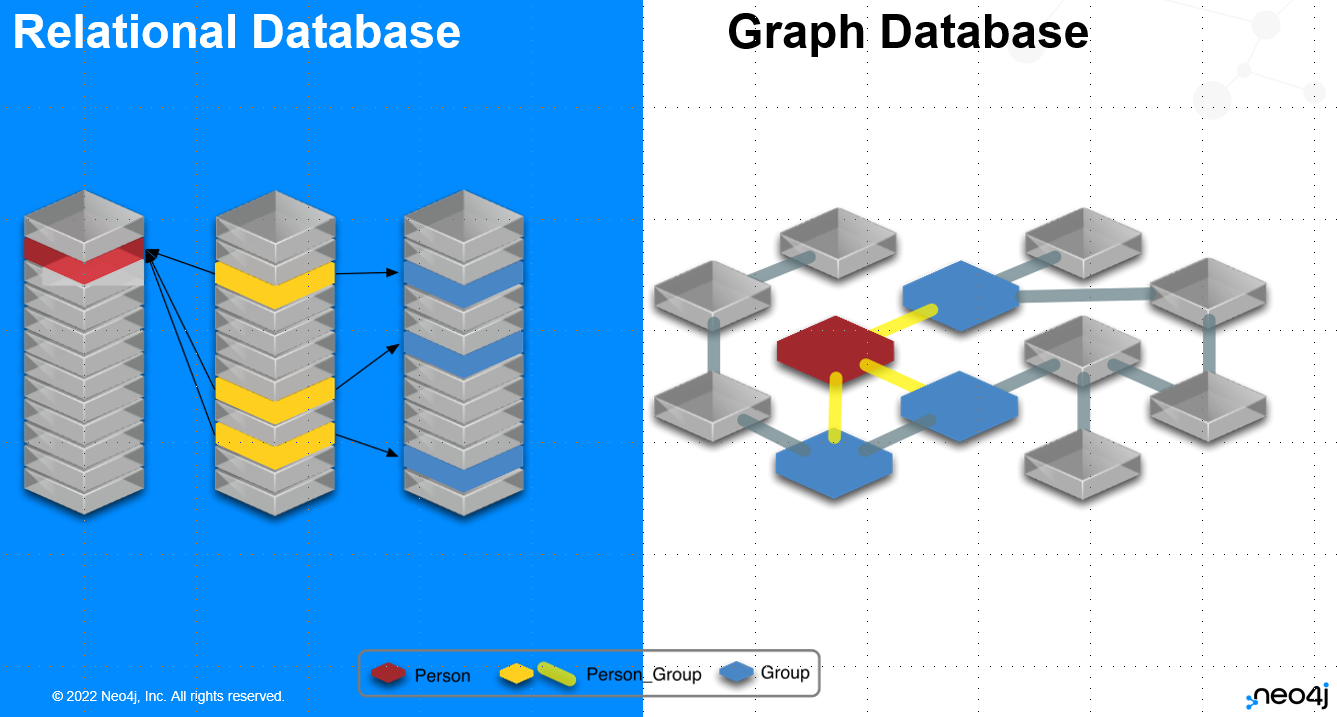
\includegraphics[width=\linewidth,keepaspectratio]{neo4j111}
\end{center}	  

\end{frame}

%%%%%%%%%%%%%%%%%%%%%%%%%%%%%%%%%%%%%%%%%%%%%%%%%%%%%%%%%%%%%%%%%%%%%%%%%%%%%%%%%%
\begin{frame}[fragile]\frametitle{Neo4j: A Graph Database}
  \begin{itemize}
    \item Neo4j is a leading graph database that allows you to model, store, and query highly connected data.
    \item Features:
    \begin{itemize}
      \item Native graph storage and processing
      \item Cypher query language
      \item ACID transactions
      \item High scalability and performance
    \end{itemize}
    \item Neo4j provides a flexible and efficient way to work with graph data.
  \end{itemize}
\end{frame}

%%%%%%%%%%%%%%%%%%%%%%%%%%%%%%%%%%%%%%%%%%%%%%%%%%%%%%%%%%%%%%%%%%%%%%%%%%%%%%%%%%
\begin{frame}[fragile]\frametitle{What is Neo4j?}
  \begin{itemize}
    \item Idea conceived on a flight to Mumbai
    \item Product \& Company started in 2007
    \item Open-Core Model:
    \begin{itemize}
      \item Free Open-Source Community Edition
      \item Closed-Source Enterprise Edition
    \end{itemize}
    \item Free for local use with Neo4j Desktop / Docker
	\item Current Version: 5.0 (Released in Nov 2022)
  \end{itemize}
\end{frame}


%%%%%%%%%%%%%%%%%%%%%%%%%%%%%%%%%%%%%%%%%%%%%%%%%%%%%%%%%%%%%%%%%%%%%%%%%%%%%%%%%%
\begin{frame}[fragile]\frametitle{Graph Database Use Cases}
  \begin{itemize}
    \item Fraud detection and prevention
    \item Social network analysis
    \item Recommendation engines
    \item Network and IT operations
    \item Knowledge graph management
    \item Impact analysis and risk assessment
    \item Master data management
    \item And many more!
  \end{itemize}
\end{frame}

%%%%%%%%%%%%%%%%%%%%%%%%%%%%%%%%%%%%%%%%%%%%%%%%%%%%%%%%%%%%%%%%%%%%%%%%%%%%%%%%%%
\begin{frame}[fragile]\frametitle{Graph Modeling in Neo4j}
  \begin{itemize}
    \item Neo4j follows a property graph model.
    \item Nodes represent entities, while relationships capture the connections between them.
    \item Nodes and relationships can have properties to store additional information.
    \item Labels and relationship types provide meaningful categorization.
  \end{itemize}
\end{frame}

%%%%%%%%%%%%%%%%%%%%%%%%%%%%%%%%%%%%%%%%%%%%%%%%%%%%%%%%%%%%%%%%%%%%%%%%%%%%%%%%%%
\begin{frame}[fragile]\frametitle{Cypher Query Language}
  \begin{itemize}
    \item Cypher is Neo4j's query language designed specifically for working with graph data.
    \item It is a declarative language that allows you to express complex graph patterns and operations.
    \item Cypher provides a human-readable syntax for querying and manipulating graph data.
    \item Examples of Cypher queries: CREATE, MATCH, WHERE, RETURN, etc.
  \end{itemize}
  
\begin{center}
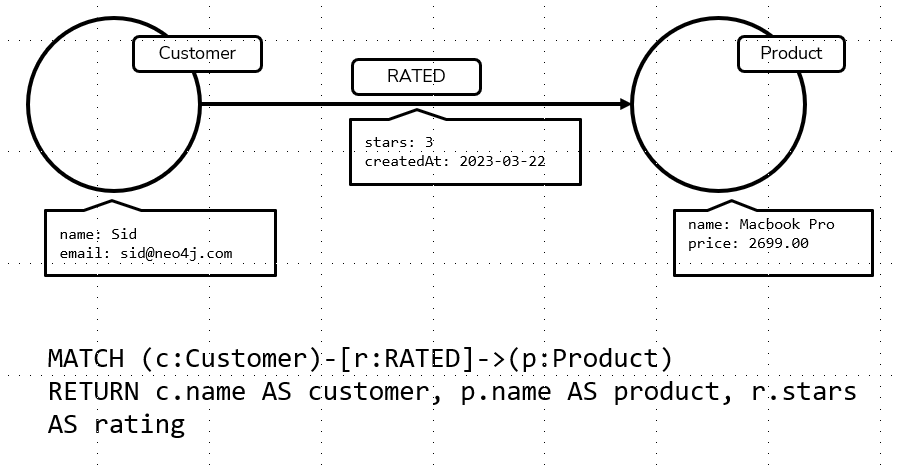
\includegraphics[width=0.8\linewidth,keepaspectratio]{neo4j108}
\end{center}	  


\end{frame}

%%%%%%%%%%%%%%%%%%%%%%%%%%%%%%%%%%%%%%%%%%%%%%%%%%%%%%%%%%%%%%%%%%%%%%%%%%%%%%%%%%
\begin{frame}[fragile]\frametitle{Nodes and relationships at a glance}

\begin{center}
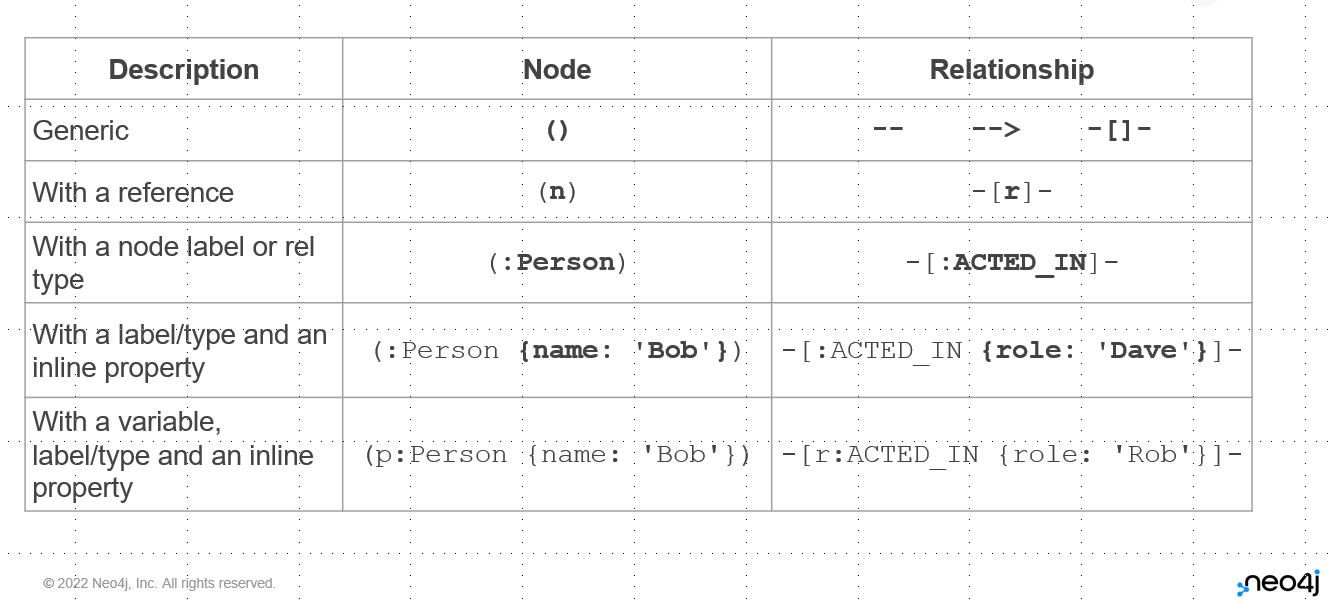
\includegraphics[width=\linewidth,keepaspectratio]{neo4j109}
\end{center}	  


\end{frame}

%%%%%%%%%%%%%%%%%%%%%%%%%%%%%%%%%%%%%%%%%%%%%%%%%%%%%%%%%%%%%%%%%%%%%%%%%%%%%%%%%%
\begin{frame}[fragile]\frametitle{Graph Data Import}
  \begin{itemize}
    \item To work with graph data in Neo4j, you need to import it into the graph database.
    \item Neo4j provides various methods for data import, including:
    \begin{itemize}
      \item CSV import: Bulk import data from CSV files.
      \item Integration with ETL (Extract, Transform, Load) tools.
      \item Integration with programming languages (e.g., Java, Python) using Neo4j drivers.
    \end{itemize}
    \item Efficient data import is crucial for graph analytics workflows.
  \end{itemize}
\end{frame}

%%%%%%%%%%%%%%%%%%%%%%%%%%%%%%%%%%%%%%%%%%%%%%%%%%%%%%%%%%%%%%%%%%%%%%%%%%%%%%%%%%
\begin{frame}[fragile]\frametitle{Graph Analytics Workflow}
  \begin{itemize}
    \item Define the problem: Identify the business problem that can be solved using graph analytics.
    \item Data modeling: Create a graph data model that represents the problem domain.
    \item Data import: Import data into the graph database.
    \item Algorithm selection: Choose the appropriate graph algorithm(s) for the problem at hand.
    \item Algorithm execution: Run the selected algorithm(s) on the graph data.
    \item Result interpretation: Analyze and interpret the algorithm output to gain insights.
  \end{itemize}
\end{frame}



%%%%%%%%%%%%%%%%%%%%%%%%%%%%%%%%%%%%%%%%%%%%%%%%%%%%%%%%%%%%%%%%%%%%%%%%%%%%%%%%%%
\begin{frame}[fragile]\frametitle{Neo4j Architecture}
  \begin{center}
    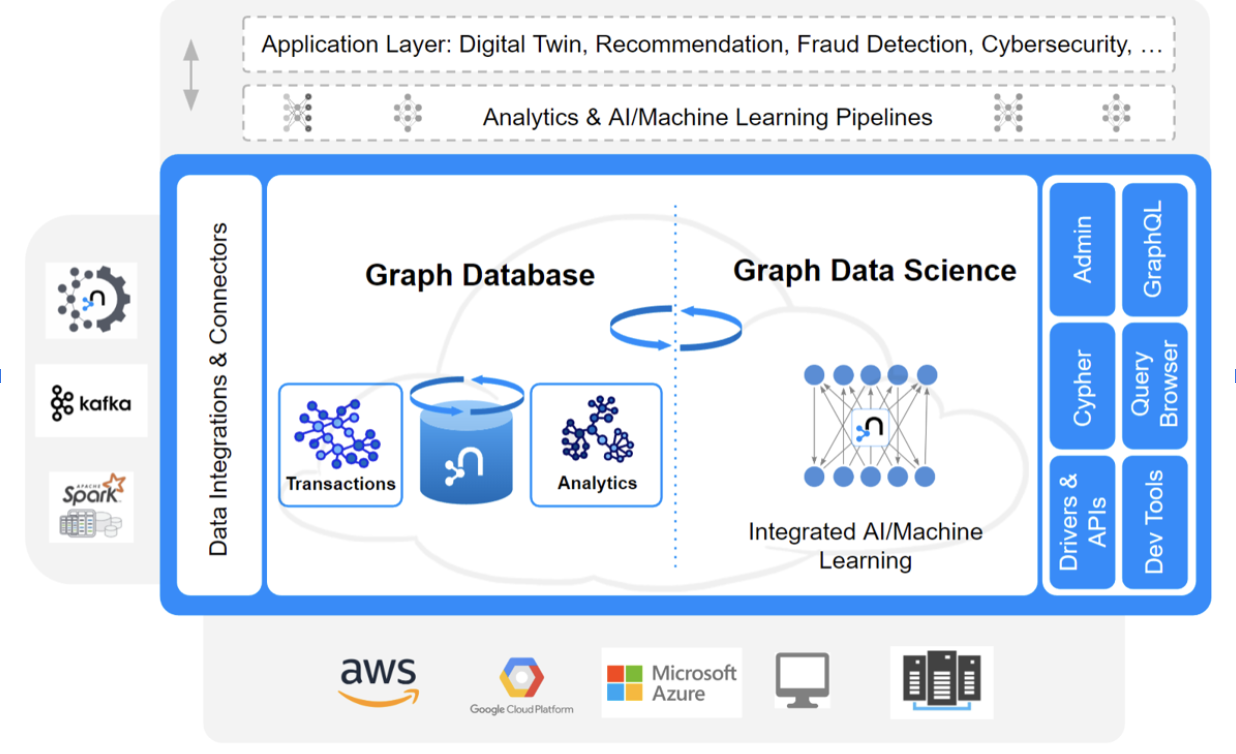
\includegraphics[width=0.6\textwidth]{neo4j_architecture.png}
	
	{\tiny (Ref: https://neo4j.com/blog/neo4j-integrates-data-ecosystem-connectors/)}
	
  \end{center}
  \begin{itemize}
    \item Neo4j follows a client-server architecture.
    \item Core components: Graph engine, transaction manager, and query processing.
    \item Highly scalable and fault-tolerant architecture.
  \end{itemize}
\end{frame}


%%%%%%%%%%%%%%%%%%%%%%%%%%%%%%%%%%%%%%%%%%%%%%%%%%%%%%%%%%%%%%%%%%%%%%%%%%%%%%%%%%
\begin{frame}[fragile]\frametitle{Scalability and Performance}
  \begin{itemize}
    \item Neo4j is designed to handle large-scale graph datasets.
    \item It provides horizontal scalability through clustering and sharding techniques.
    \item Queries are optimized for efficient graph traversal and pattern matching.
    \item Neo4j's query optimizer maximizes query performance.
  \end{itemize}
\end{frame}

\section[GDS]{Graph Data Science}

%%%%%%%%%%%%%%%%%%%%%%%%%%%%%%%%%%%%%%%%%%%%%%%%%%%%%%%%%%%%%%%%%%%%%%%%%%%%%%%%%%
\begin{frame}[fragile]\frametitle{Graph Data Science}

\begin{center}
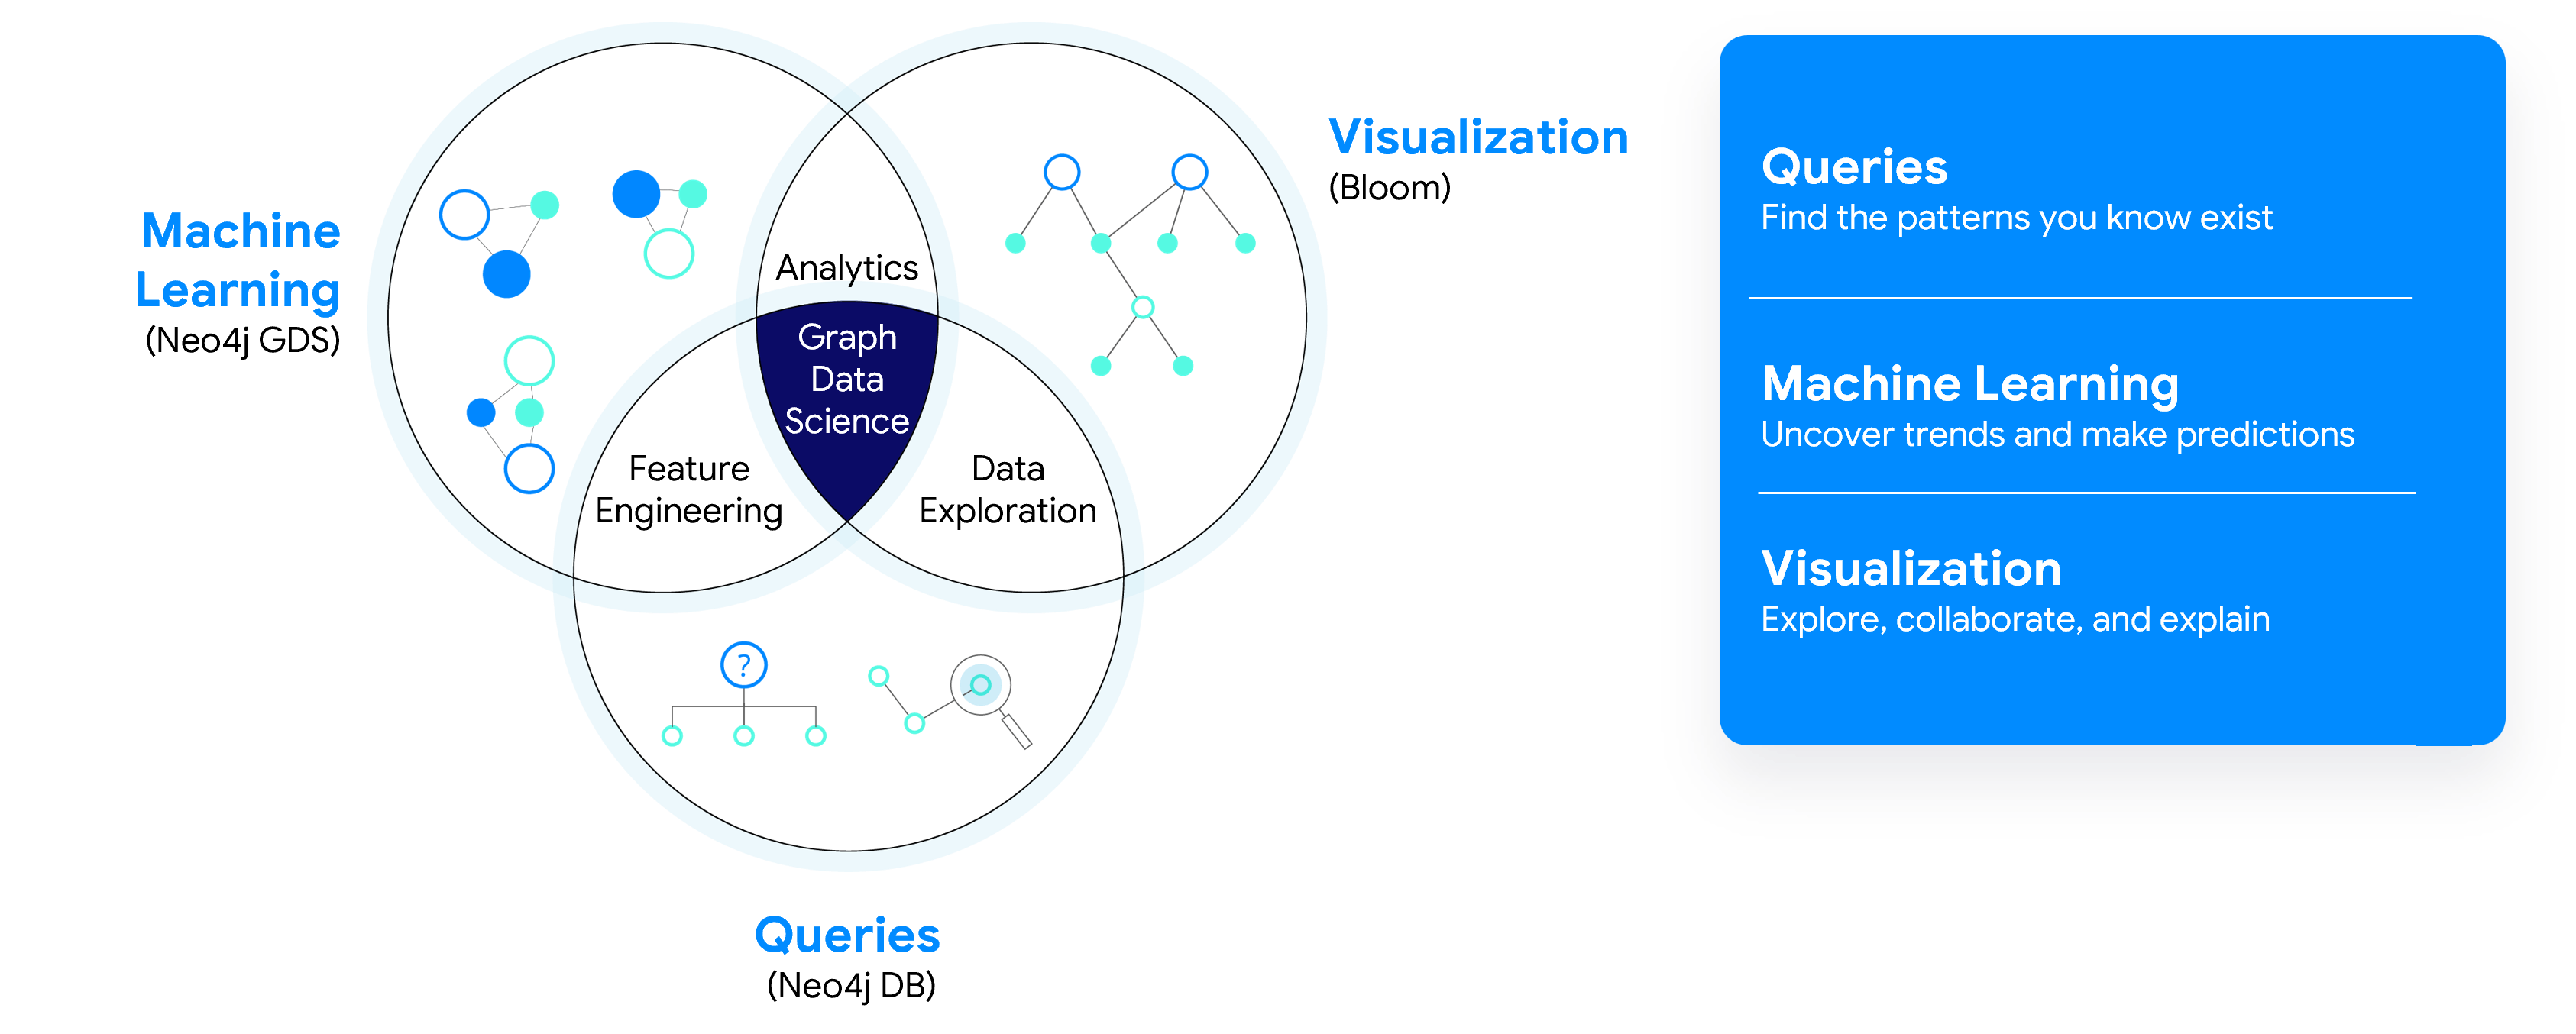
\includegraphics[width=\linewidth,keepaspectratio]{neo4j112}
\end{center}	  

\end{frame}

%%%%%%%%%%%%%%%%%%%%%%%%%%%%%%%%%%%%%%%%%%%%%%%%%%%%%%%%%%%%%%%%%%%%%%%%%%%%%%%%%%
\begin{frame}[fragile]\frametitle{Graph and Data Science}

\begin{center}
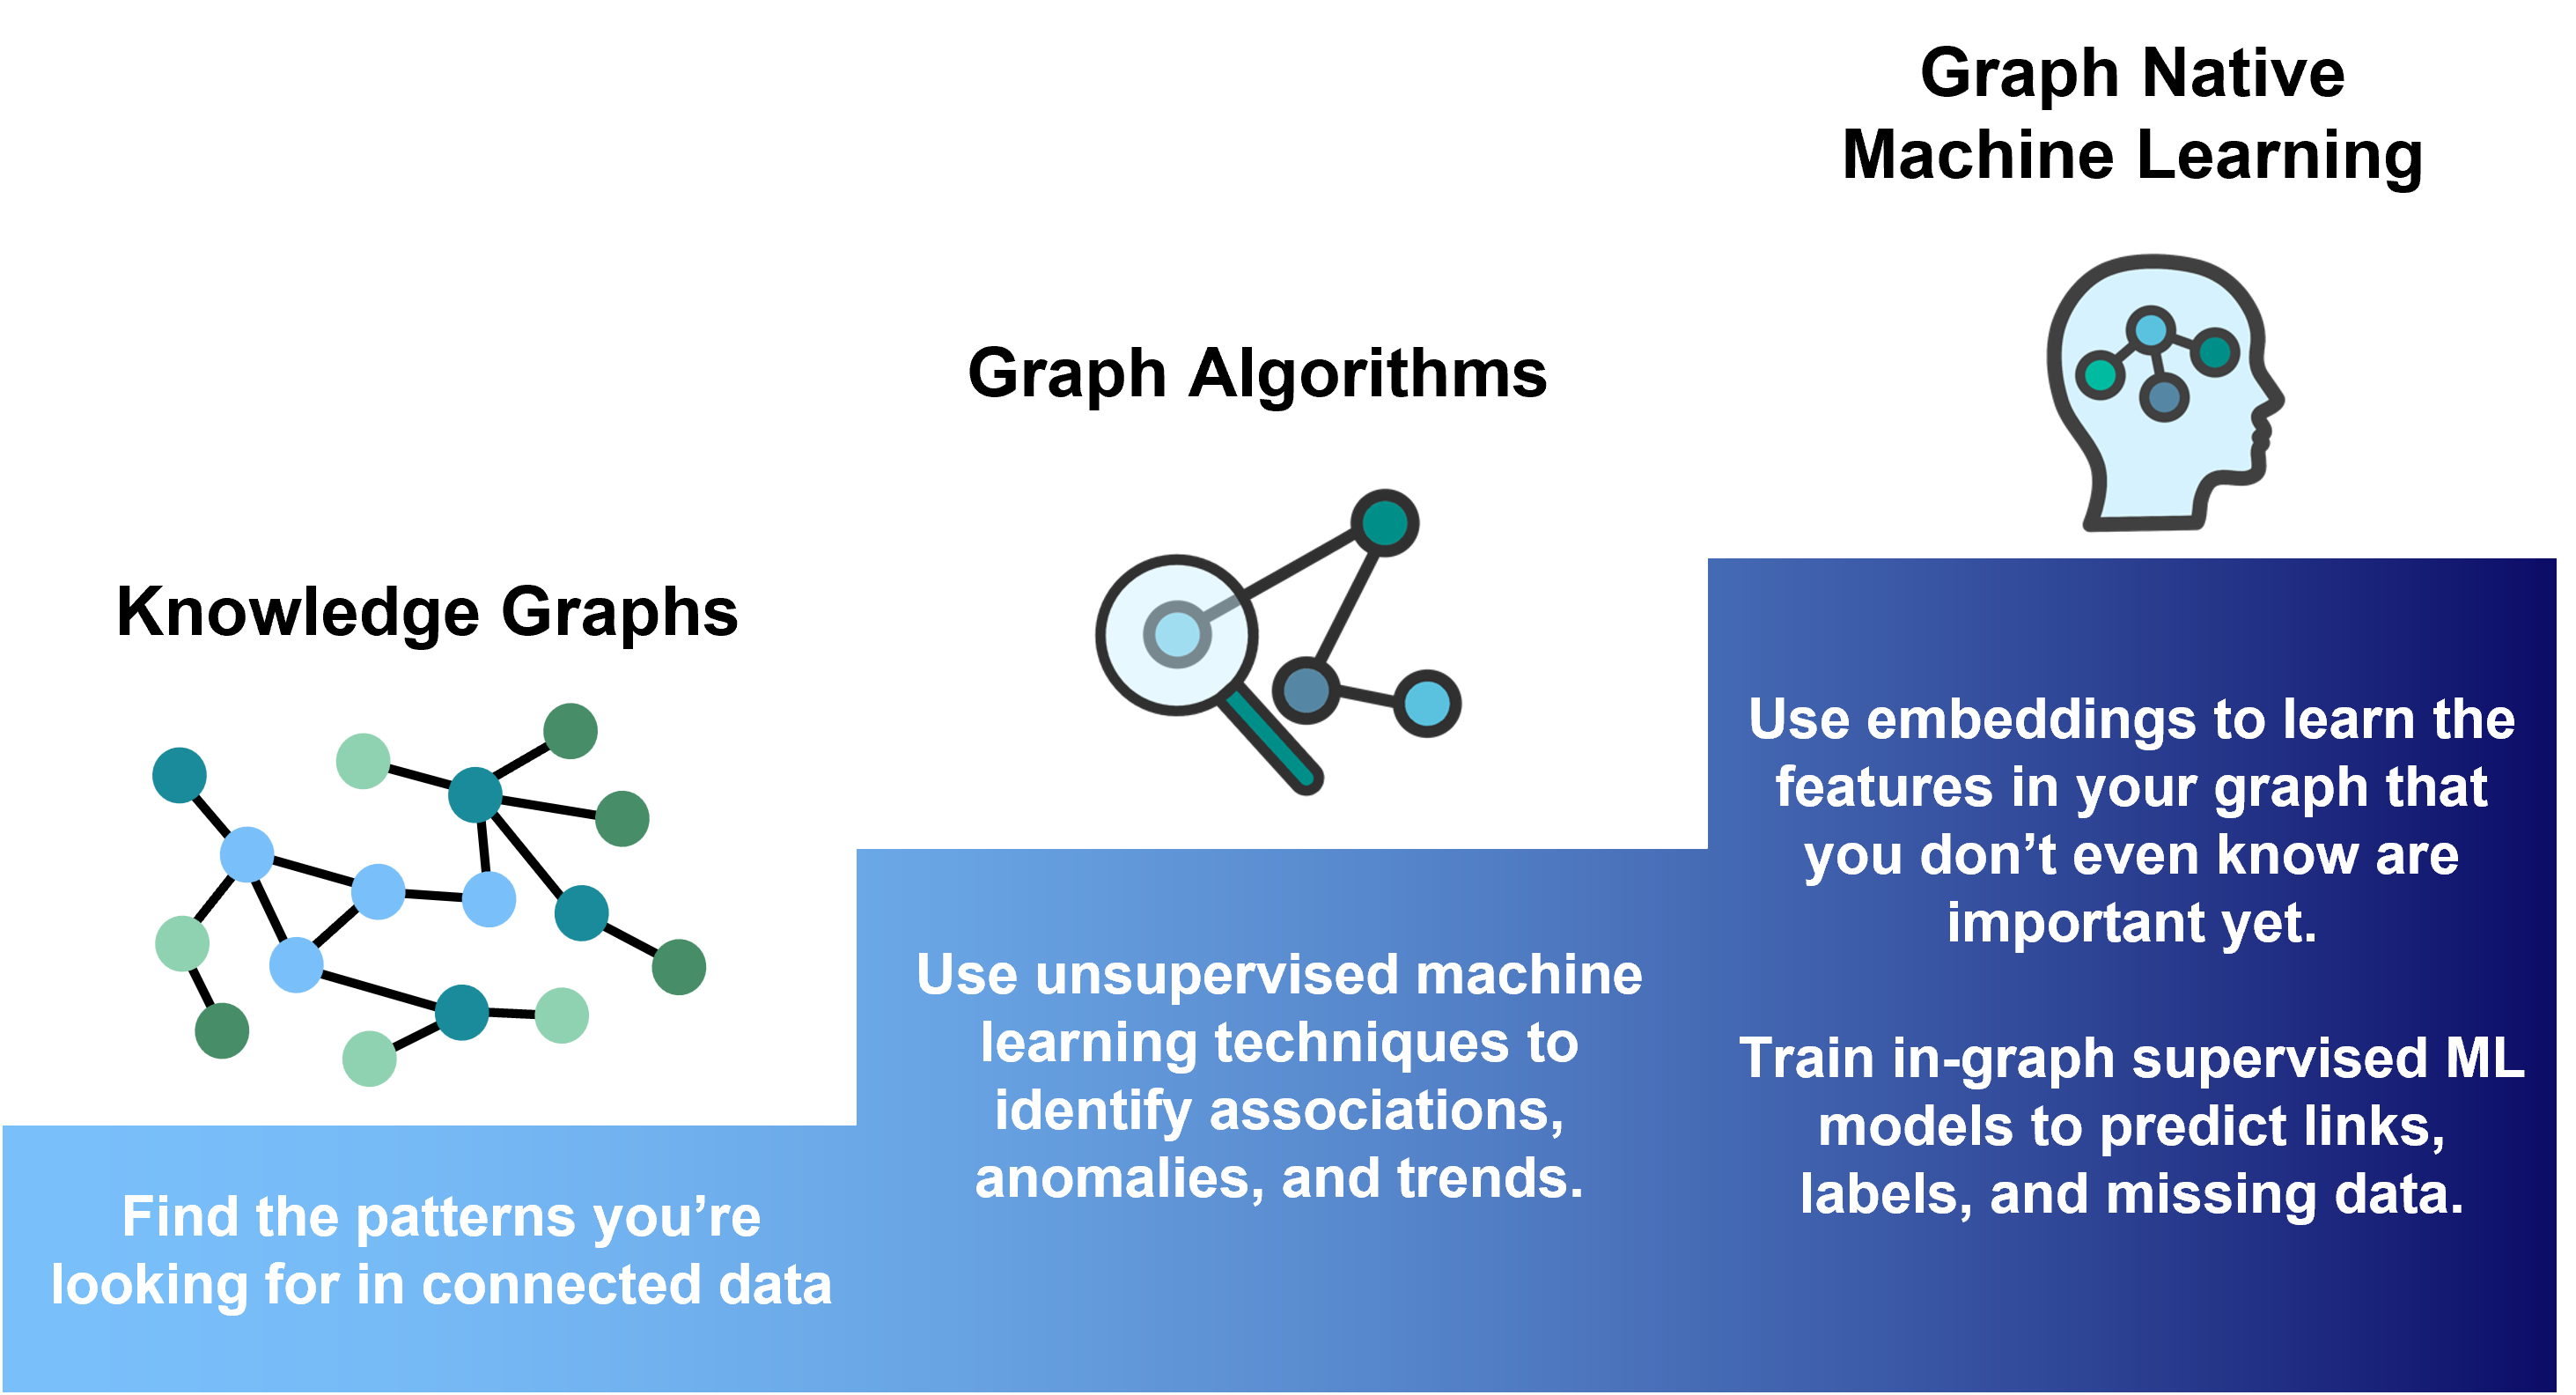
\includegraphics[width=\linewidth,keepaspectratio]{neo4j113}
\end{center}	  

\end{frame}

%%%%%%%%%%%%%%%%%%%%%%%%%%%%%%%%%%%%%%%%%%%%%%%%%%%%%%%%%%%%%%%%%%%%%%%%%%%%%%%%%%
\begin{frame}[fragile]\frametitle{Graph Data Science (GDS) Family of Algorithms}

\begin{center}
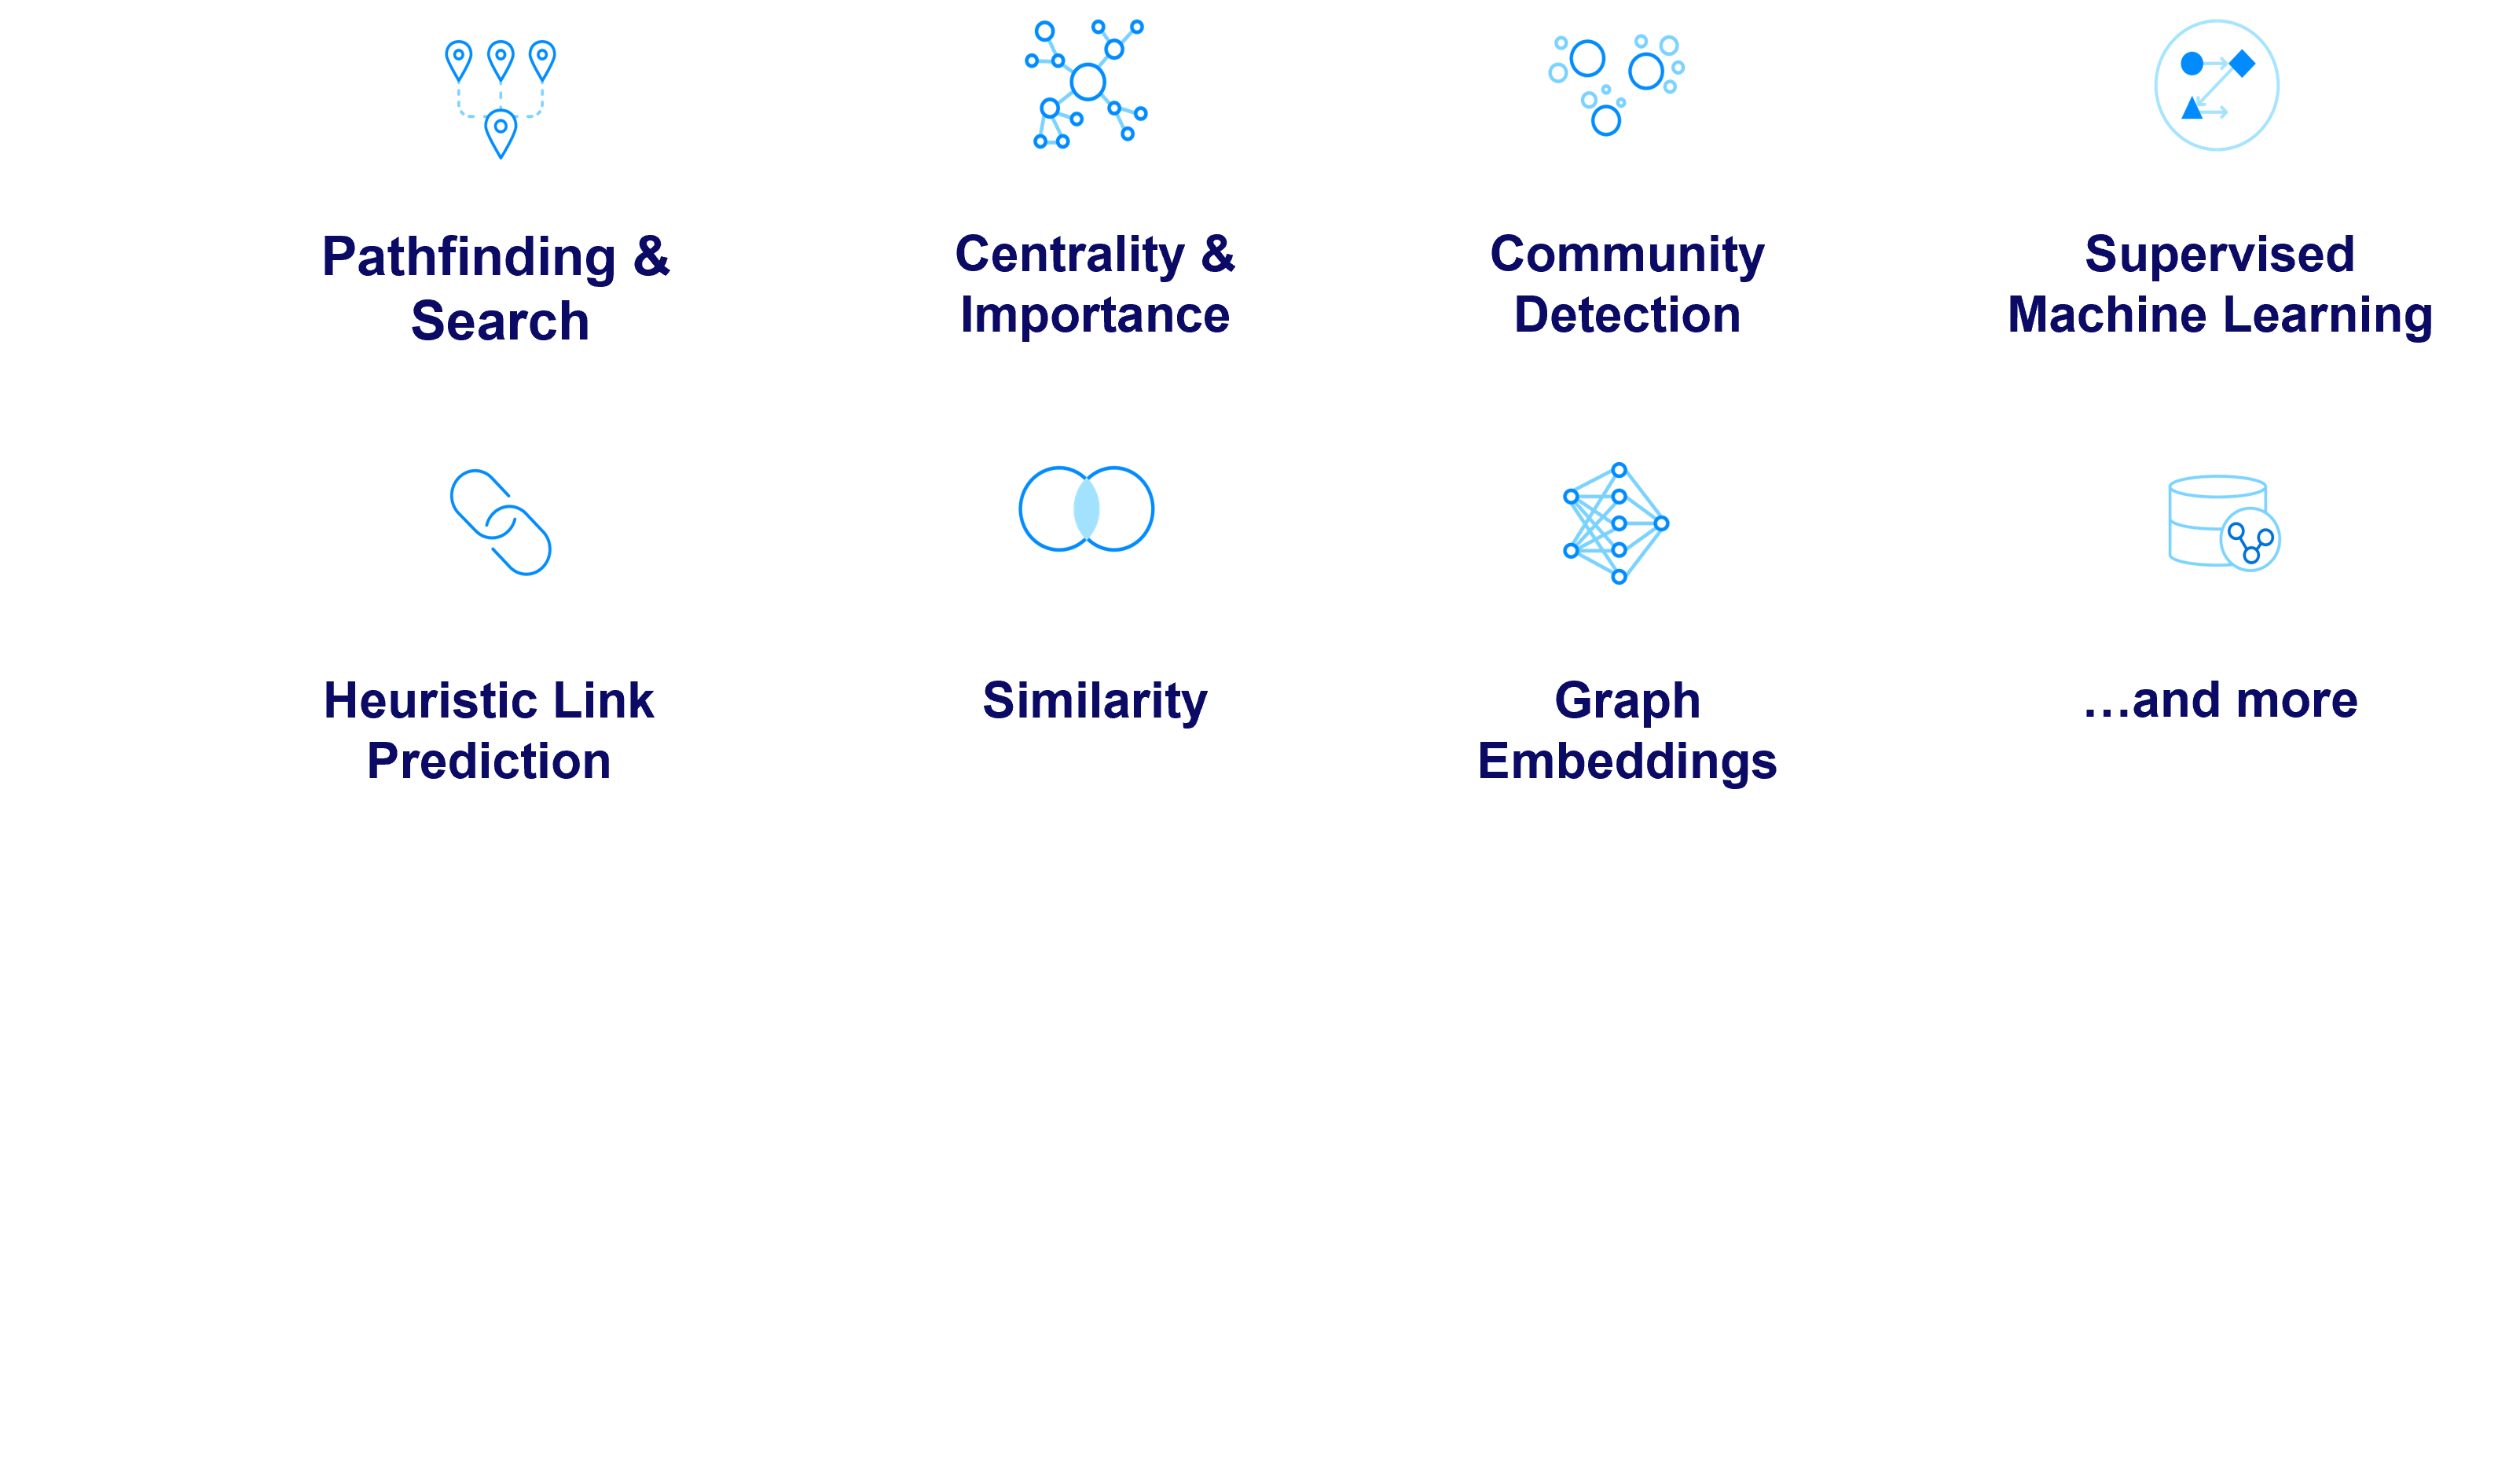
\includegraphics[width=\linewidth,keepaspectratio]{neo4j114}
\end{center}	  

\end{frame}

%%%%%%%%%%%%%%%%%%%%%%%%%%%%%%%%%%%%%%%%%%%%%%%%%%%%%%%%%%%%%%%%%%%%%%%%%%%%%%%%%%
\begin{frame}[fragile]\frametitle{GDS Process in Neo4j}

\begin{center}
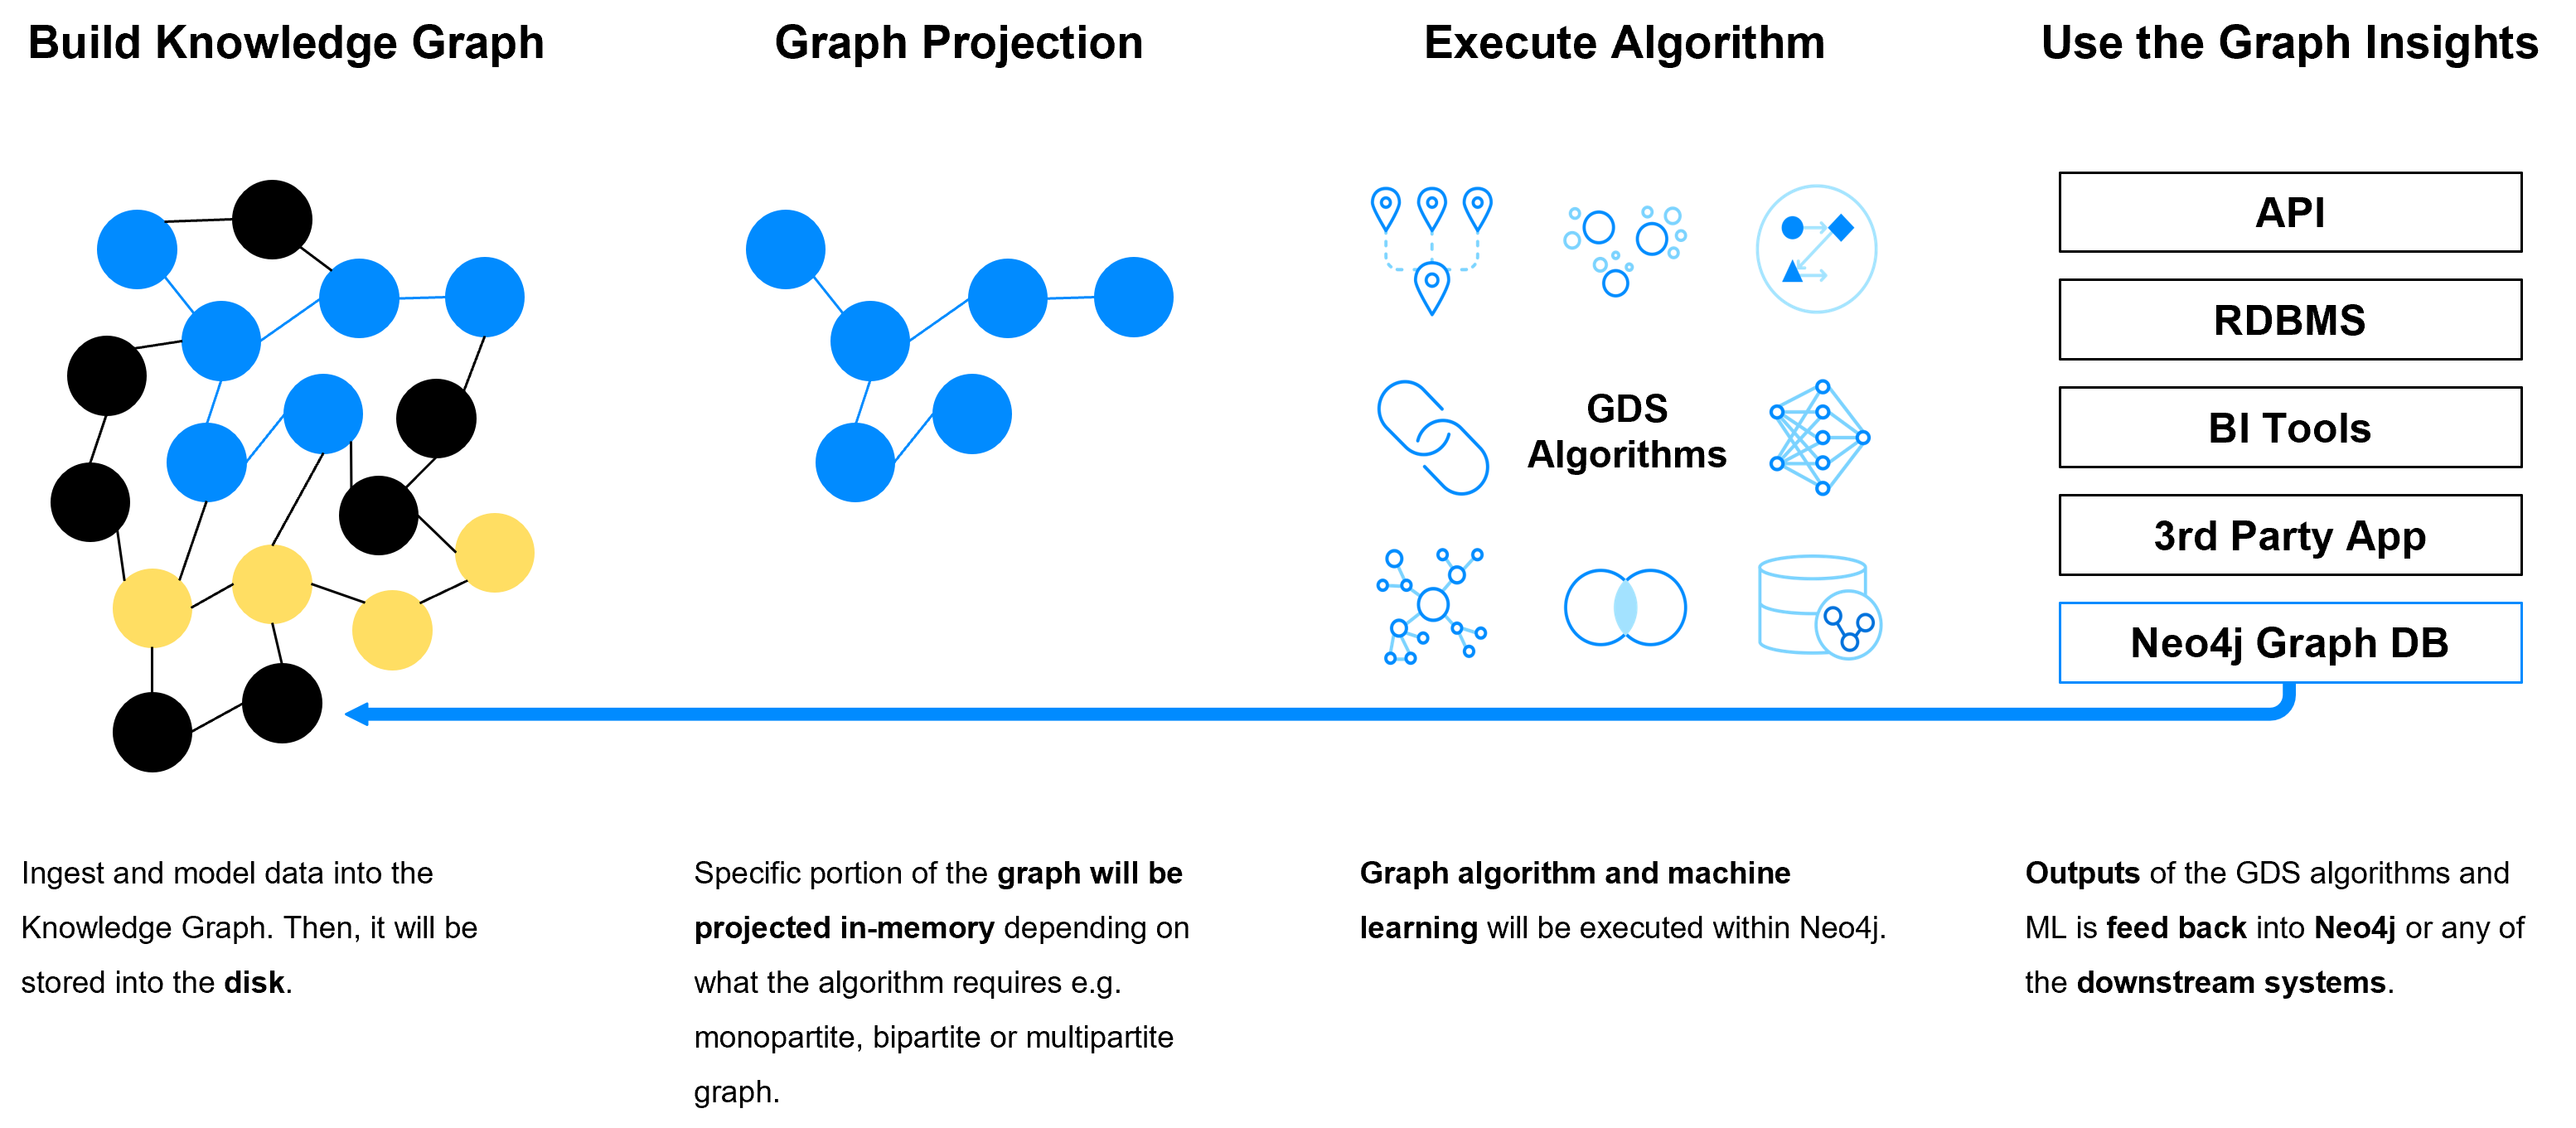
\includegraphics[width=\linewidth,keepaspectratio]{neo4j115}
\end{center}	  

\end{frame}


%%%%%%%%%%%%%%%%%%%%%%%%%%%%%%%%%%%%%%%%%%%%%%%%%%%%%%%%%%%%%%%%%%%%%%%%%%%%%%%%%%
\begin{frame}[fragile]\frametitle{Neo4j in the Google Cloud Ecosystem}

\begin{center}
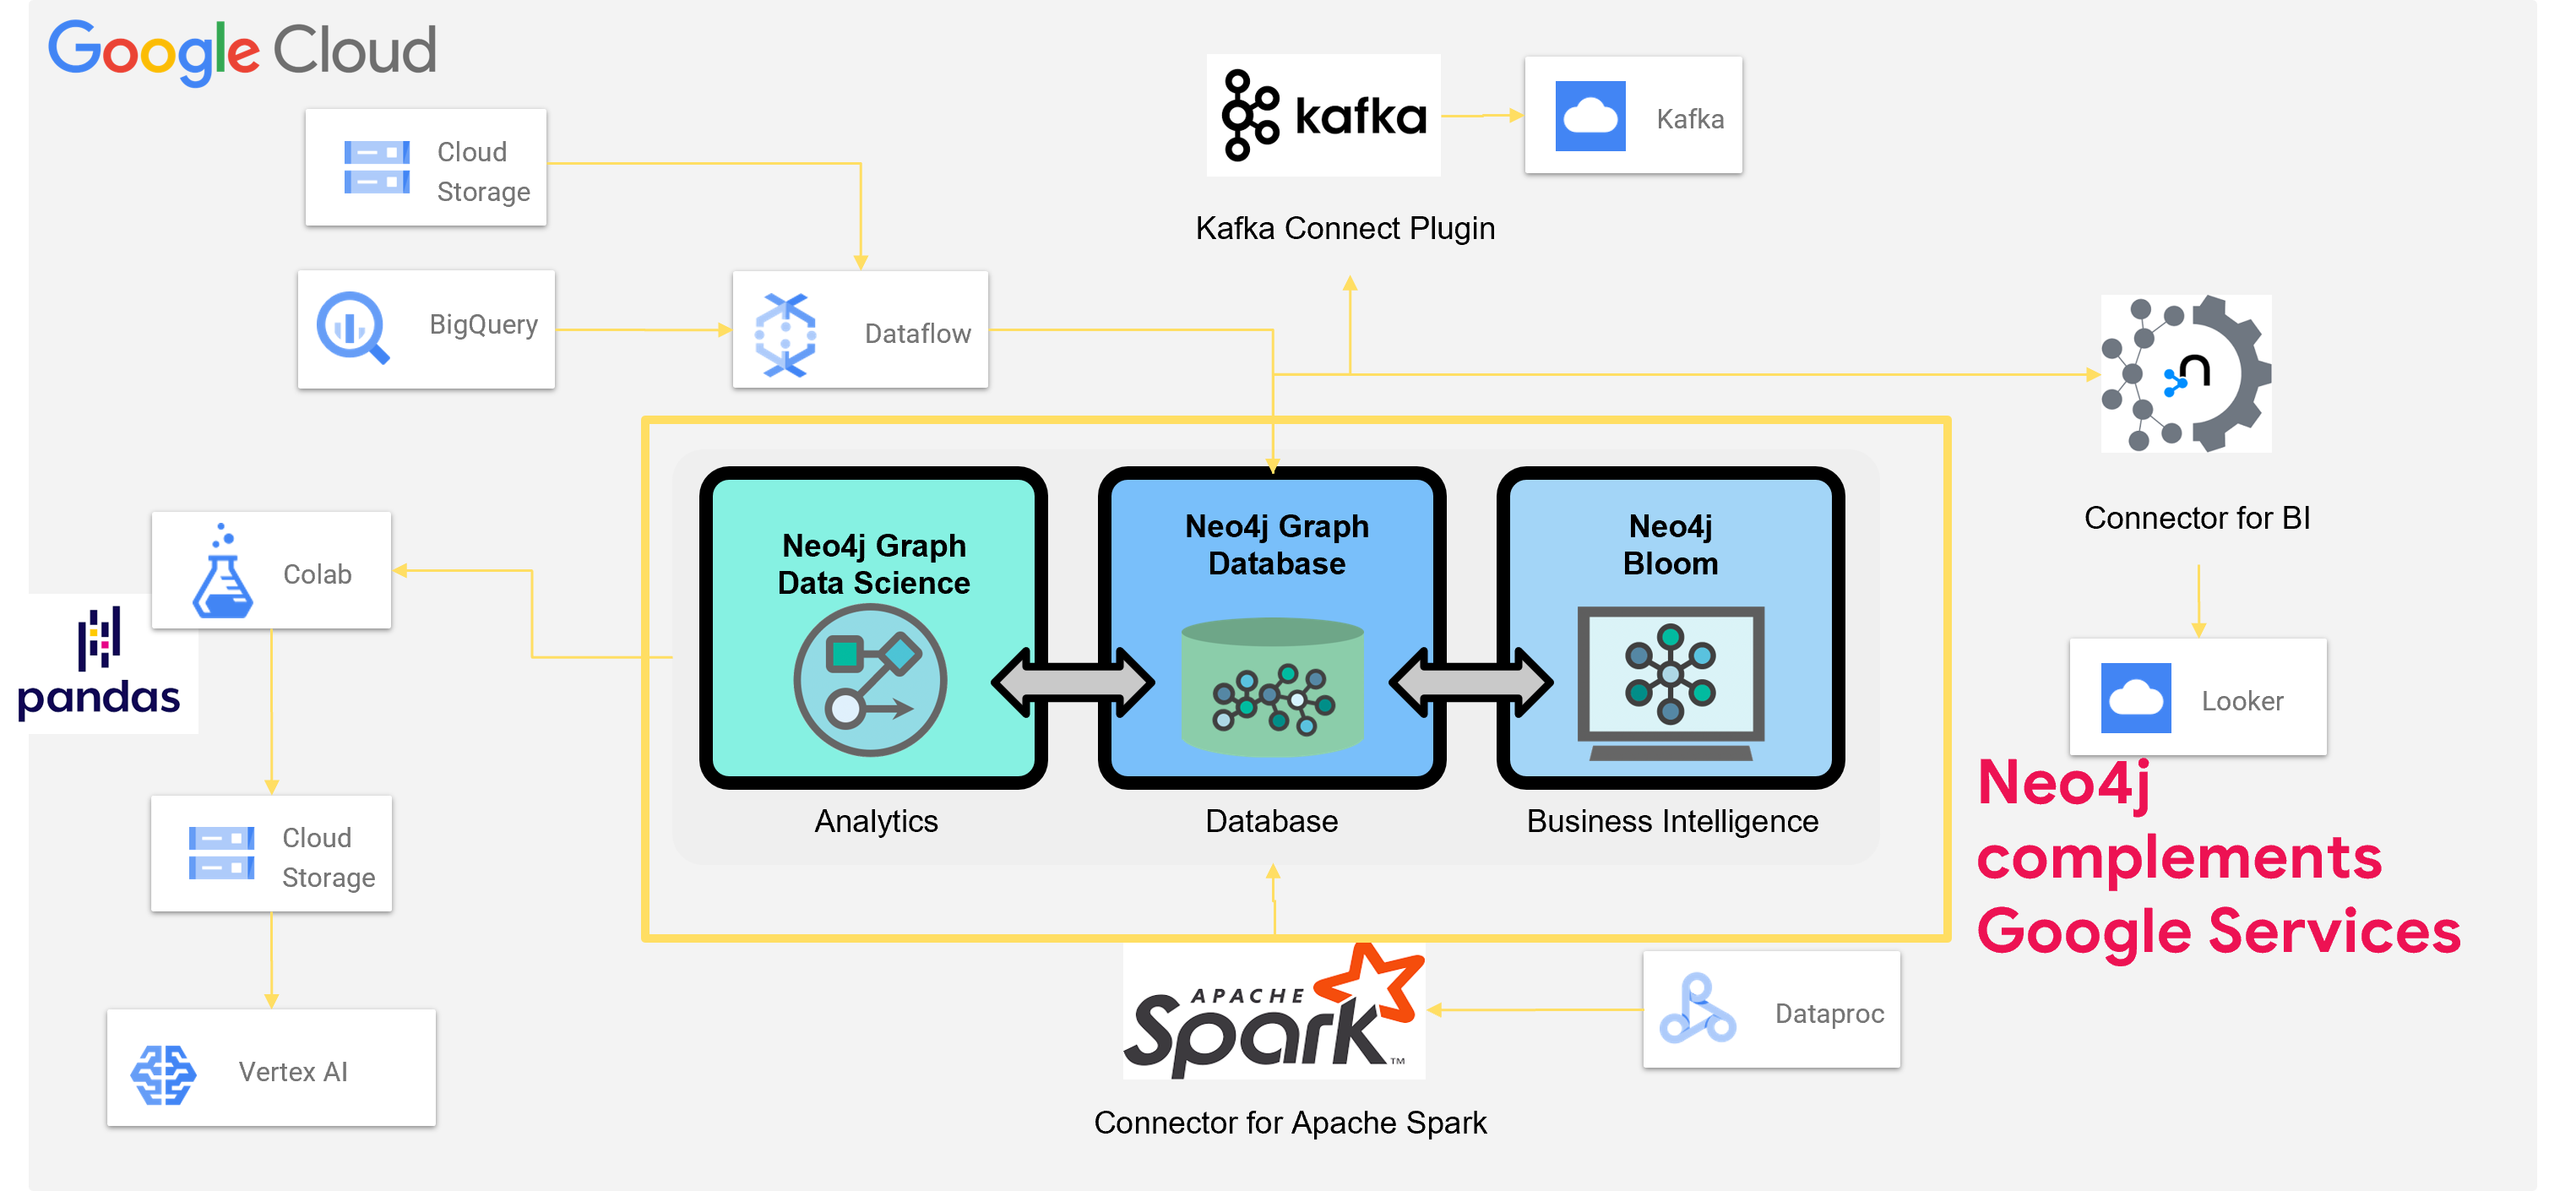
\includegraphics[width=\linewidth,keepaspectratio]{neo4j116}
\end{center}	  

\end{frame}





%%%%%%%%%%%%%%%%%%%%%%%%%%%%%%%%%%%%%%%%%%%%%%%%%%%%%%%%%%%%%%%%%%%%%%%%%%%%%%%%%%
\begin{frame}[fragile]\frametitle{Use Cases for Graph Databases}
  \begin{itemize}
    \item Fraud detection and prevention: Uncover patterns of fraudulent activities in financial transactions.
    \item Social network analysis: Identify communities, influencers, and relationships within a social graph.
    \item Recommendation engines: Power personalized recommendations based on user preferences and graph connections.
    \item Network and IT operations: Analyze and optimize network infrastructure, detect anomalies, and troubleshoot issues.
    \item Knowledge graph management: Organize and link diverse knowledge sources for semantic search and data integration.
	\item Impact analysis and risk assessment: Analyze the impact of changes or events on interconnected systems and assess associated risks.
	\item Master data management: Manage and integrate complex relationships within master data domains.
	\item Recommendation engines: Power personalized recommendations based on user preferences and graph connections.
	\item Network and IT operations: Analyze and optimize network infrastructure, detect anomalies, and troubleshoot issues.
\end{itemize}
	\end{frame}
	
%%%%%%%%%%%%%%%%%%%%%%%%%%%%%%%%%%%%%%%%%%%%%%%%%%%%%%%%%%%%%%%%%%%%%%%%%%%%%%%%%%
\begin{frame}[fragile]\frametitle{Real-World Applications}
  \begin{itemize}
    \item Healthcare: Disease networks, drug discovery
    \item E-commerce: Personalized recommendations, fraud detection
    \item Transportation: Route optimization, logistics planning
    \item Social media: Influencer analysis, community detection
    \item Finance: Anti-money laundering, fraud detection
    \item IoT: Sensor networks, anomaly detection
  \end{itemize}
\end{frame}


%%%%%%%%%%%%%%%%%%%%%%%%%%%%%%%%%%%%%%%%%%%%%%%%%%%%%%%%%%%%%%%%%%%%%%%%%%%%%%%%%%
\begin{frame}\frametitle{Common Use cases: E-Commerce Recommendations}


Easy in graph databases: those who bought A also bought B.

\begin{center}
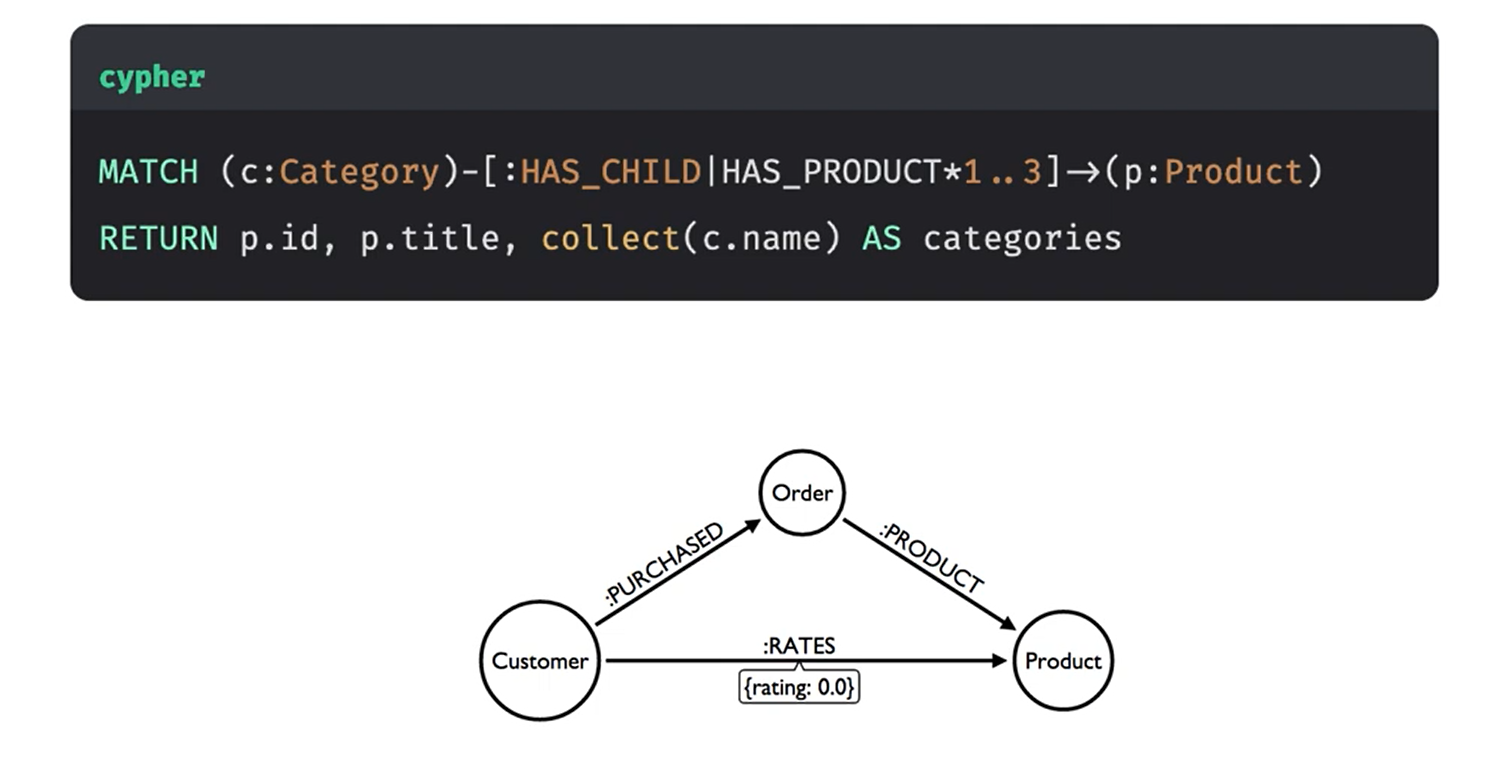
\includegraphics[width=\linewidth,keepaspectratio]{neo4j56}
\end{center}	

{\tiny (Ref: Introduction to Neo4j - a hands-on crash course - neo4j)}
\end{frame}

%%%%%%%%%%%%%%%%%%%%%%%%%%%%%%%%%%%%%%%%%%%%%%%%%%%%%%%%%%%%%%%%%%%%%%%%%%%%%%%%%%
\begin{frame}\frametitle{Common Use cases: Investigative Journalism}

Panama papers: Identify corruption based on relationships between people/companies/financial-institutions.

\begin{center}
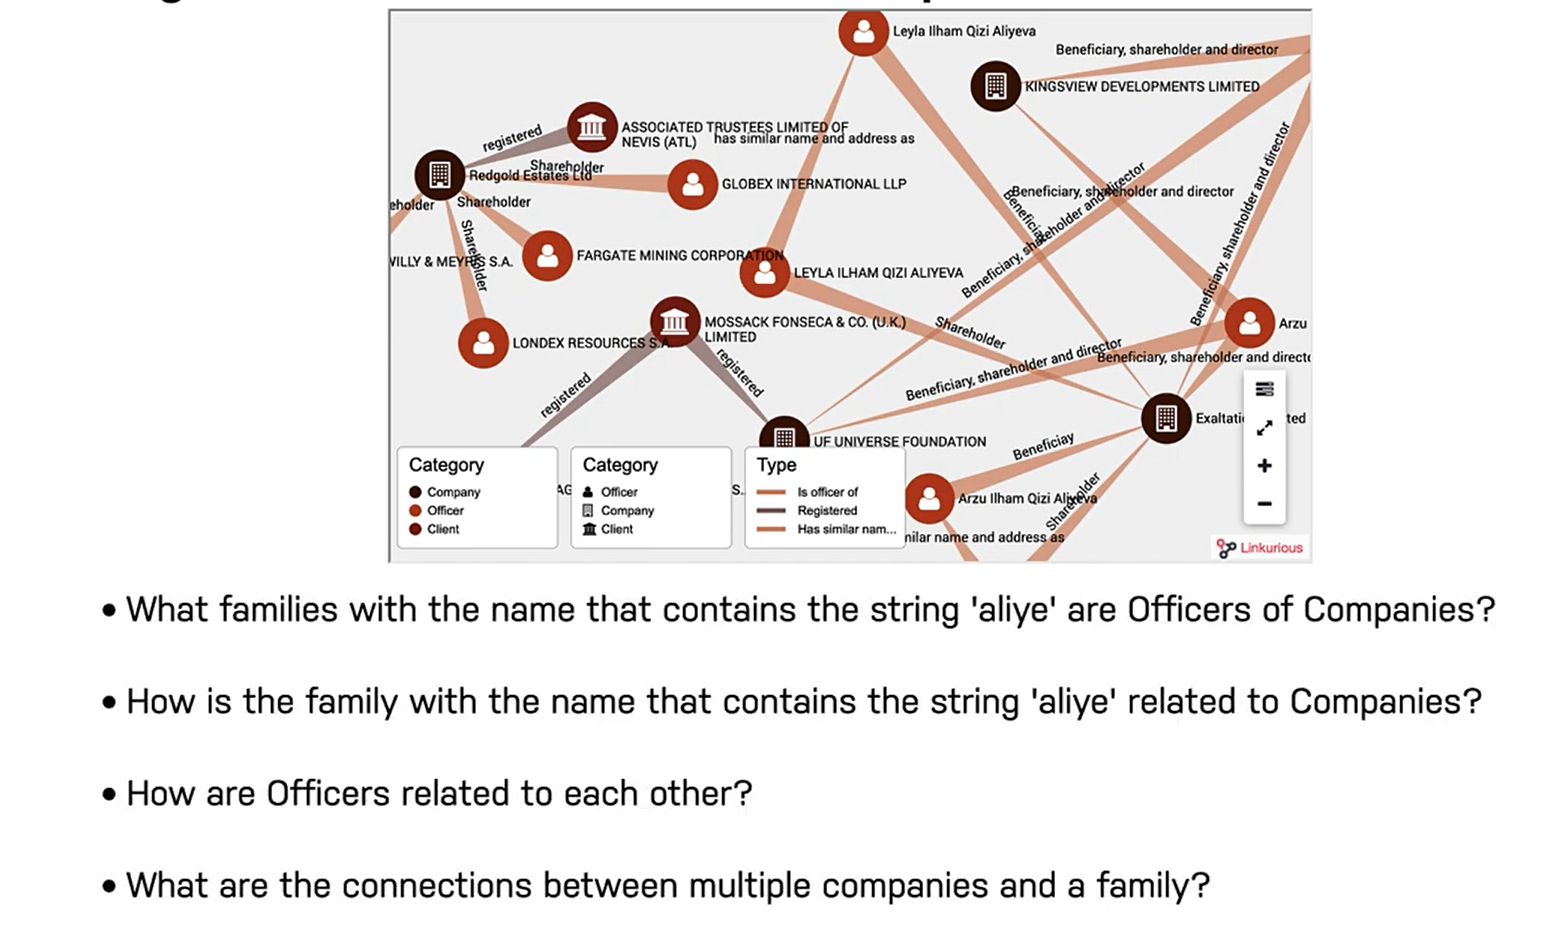
\includegraphics[width=0.8\linewidth,keepaspectratio]{neo4j57}
\end{center}	

{\tiny (Ref: Introduction to Neo4j - a hands-on crash course - neo4j)}
\end{frame}

%%%%%%%%%%%%%%%%%%%%%%%%%%%%%%%%%%%%%%%%%%%%%%%%%%%%%%%%%%%%%%%%%%%%%%%%%%%%%%%%%%
\begin{frame}[fragile]\frametitle{Common Use cases: Network Dependencies}



\begin{center}
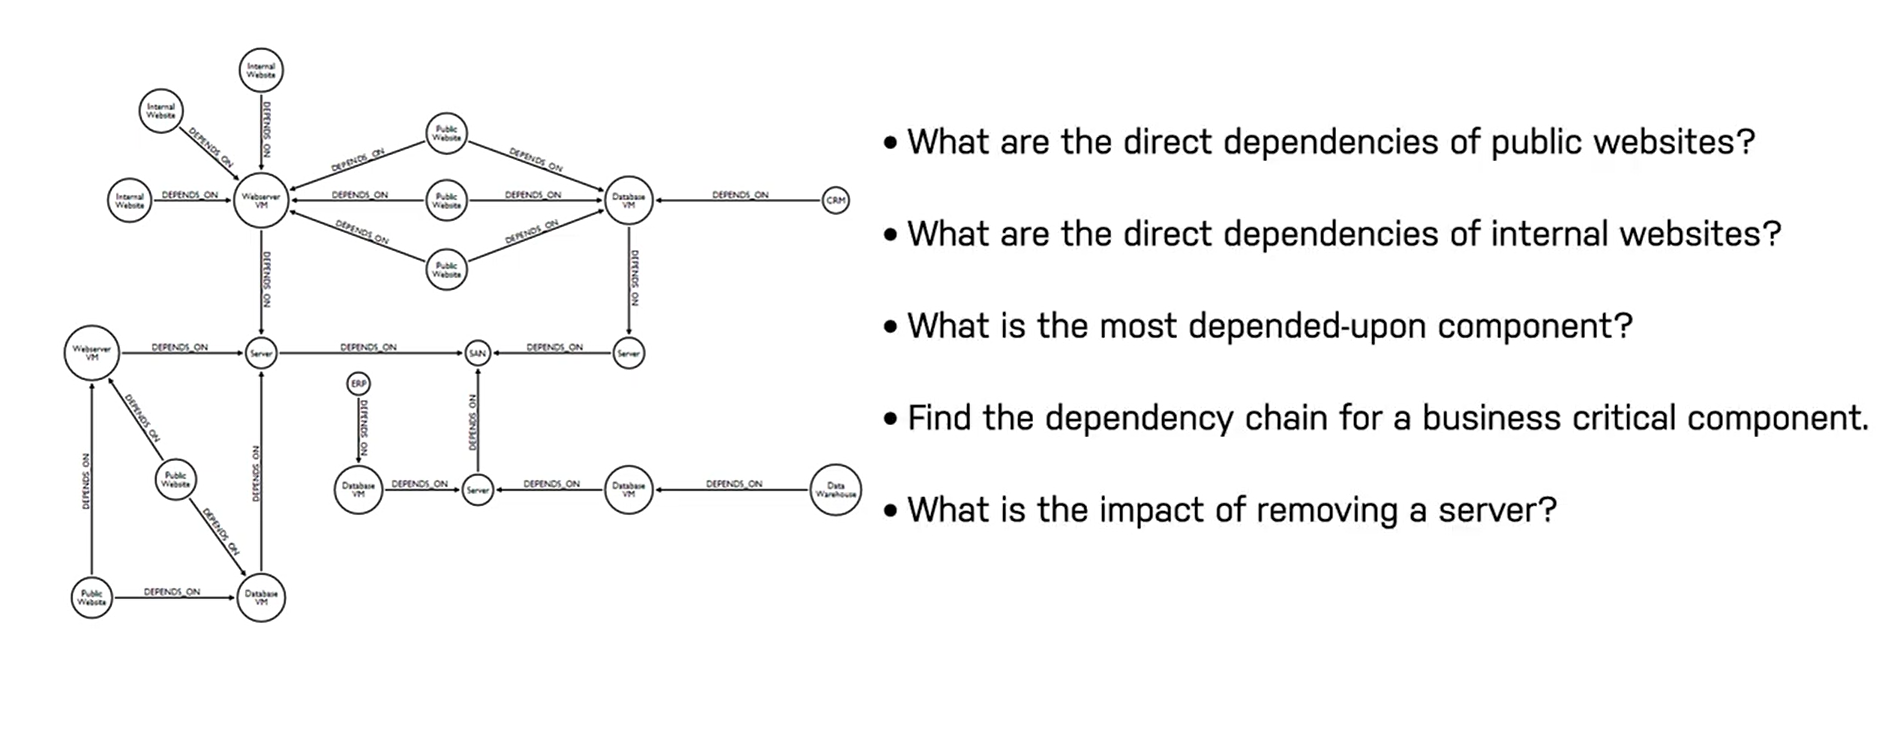
\includegraphics[width=\linewidth,keepaspectratio]{neo4j58}
\end{center}	

{\tiny (Ref: Introduction to Neo4j - a hands-on crash course - neo4j)}
\end{frame}


%%%%%%%%%%%%%%%%%%%%%%%%%%%%%%%%%%%%%%%%%%%%%%%%%%%%%%%%%%%%%%%%%%%%%%%%%%%%%%%%%%
\begin{frame}[fragile]\frametitle{Common Use cases: Supply Chain}



\begin{center}
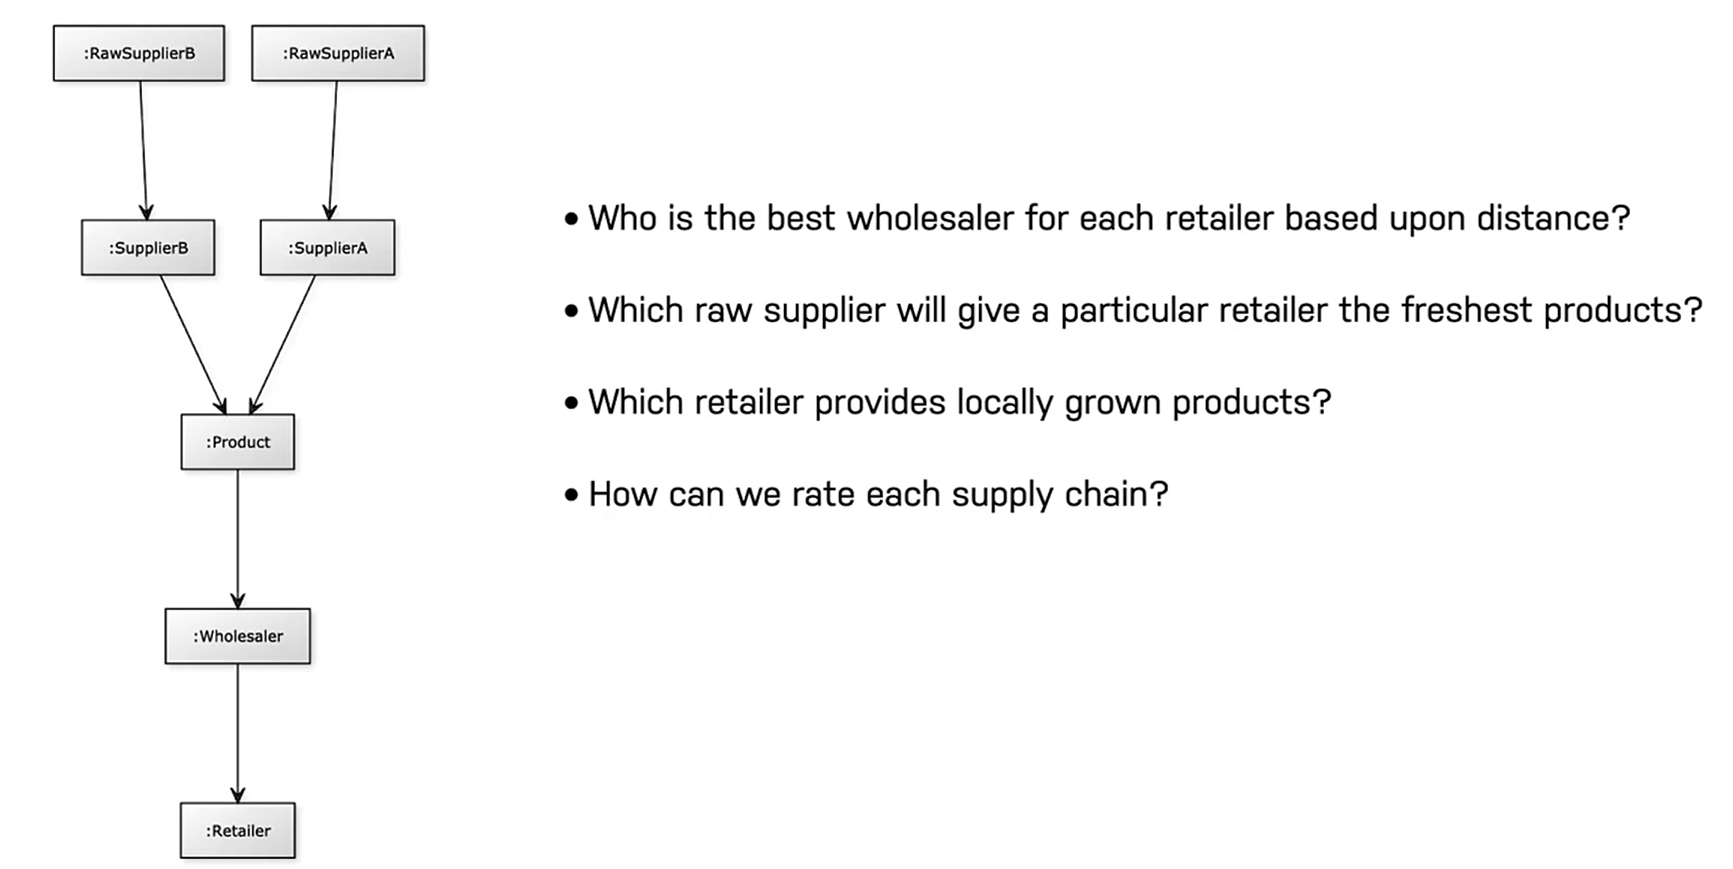
\includegraphics[width=\linewidth,keepaspectratio]{neo4j59}
\end{center}	

{\tiny (Ref: Introduction to Neo4j - a hands-on crash course - neo4j)}
\end{frame}



%%%%%%%%%%%%%%%%%%%%%%%%%%%%%%%%%%%%%%%%%%%%%%%%%%%%%%%%%%%%%%%%%%%%%%%%%%%%%%%%%%
\begin{frame}[fragile]\frametitle{}

\begin{center}
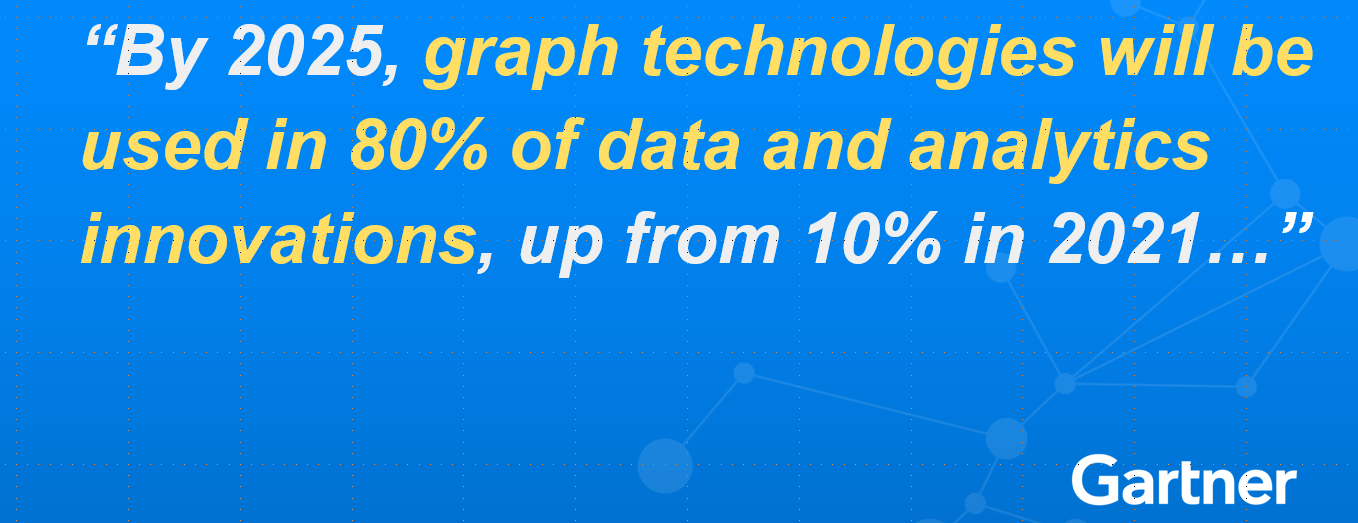
\includegraphics[width=\linewidth,keepaspectratio]{neo4j110}
\end{center}	  

\end{frame}

%%%%%%%%%%%%%%%%%%%%%%%%%%%%%%%%%%%%%%%%%%%%%%%%%%%%%%%%%%%%%%%%%%%%%%%%%%%%%%%%%%
\begin{frame}[fragile]\frametitle{Continue your graph journey with Graph Academy}

\begin{center}
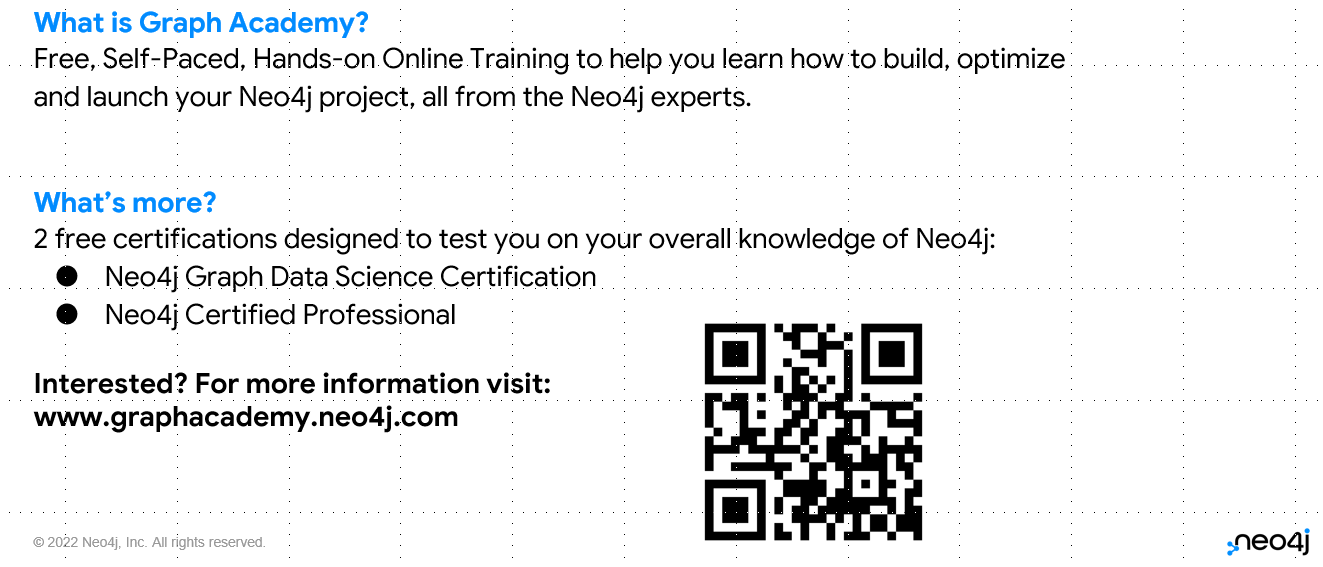
\includegraphics[width=\linewidth,keepaspectratio]{neo4j117}
\end{center}	  

\end{frame}

%%%%%%%%%%%%%%%%%%%%%%%%%%%%%%%%%%%%%%%%%%%%%%%%%%%%%%%%%%%%%%%%%%%%%%%%%%%%%%%%%%
\begin{frame}[fragile]\frametitle{Community}

\begin{center}
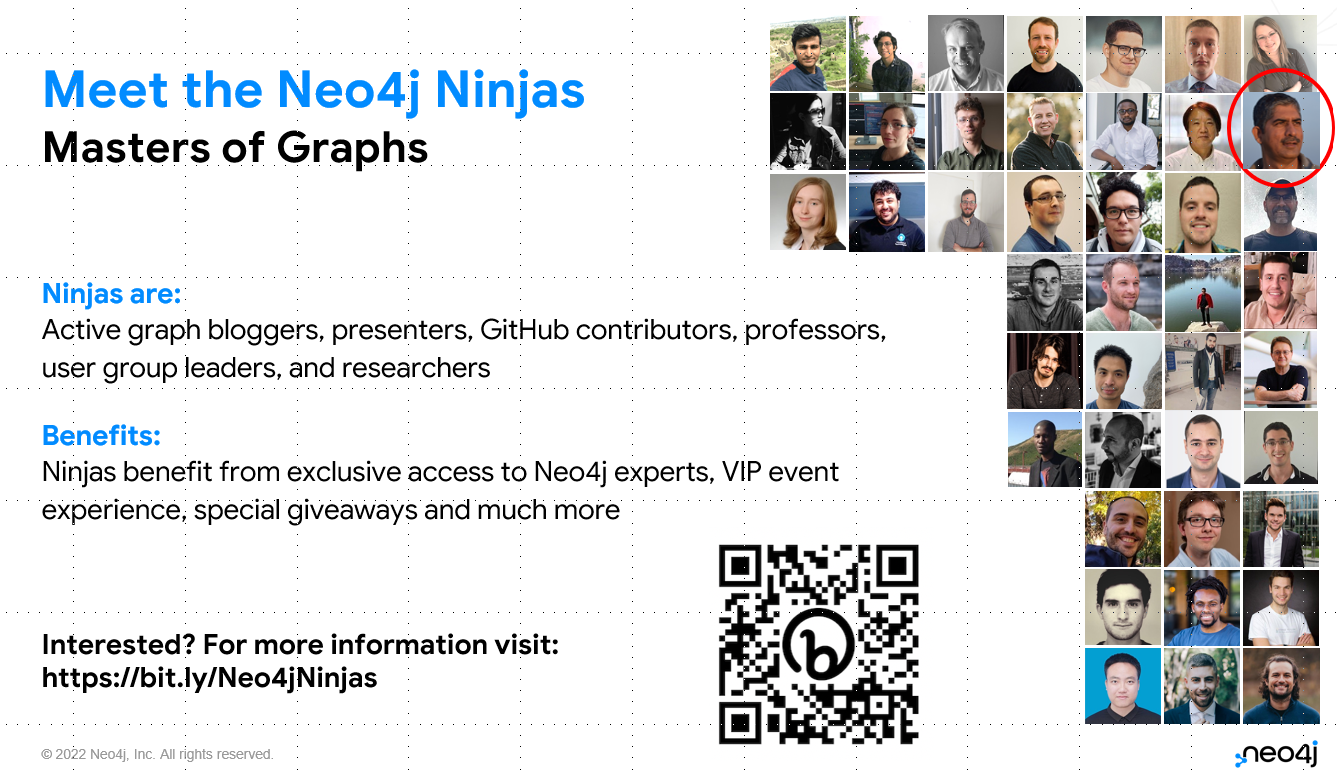
\includegraphics[width=\linewidth,keepaspectratio]{neo4j118}
\end{center}	  

\end{frame}


%%%%%%%%%%%%%%%%%%%%%%%%%%%%%%%%%%%%%%%%%%%%%%%%%%%%%%%%%%%%%%%%%%%%%%%%%%%%%%%%%%
\begin{frame}[fragile]\frametitle{Key Takeaways}
  \begin{itemize}
    \item Graphs are a natural way to represent and analyze complex relationships in various domains.
    \item Neo4j provides a powerful and efficient graph database solution for working with highly connected data.
    \item Graph algorithms enable powerful insights and solutions to a wide range of problems.
  \end{itemize}
\end{frame}

